\documentclass[11pt,a4paper]{report}
\usepackage[margin=2.3cm]{geometry}
\usepackage[T1]{fontenc}
\usepackage{lmodern}
\usepackage{amsmath,amssymb}
\usepackage{graphicx}
\usepackage{booktabs,tabularx,longtable}
\usepackage{xcolor}
\usepackage{float}
\usepackage{caption}
\usepackage{enumitem}
\usepackage{listings}
\usepackage[most]{tcolorbox}
\usepackage{microtype}
\usepackage[colorlinks=true,linkcolor=blue!50!black,urlcolor=blue!50!black,citecolor=blue!50!black]{hyperref}

\graphicspath{{../../results/figures/}{../../manas_sa/results/}}
\setlist{itemsep=2pt,topsep=4pt}
\setlength{\emergencystretch}{3em}
\setlength{\parskip}{3pt}

% ---------- code listings ----------
\definecolor{codebg}{HTML}{F6F6F3}
\definecolor{codekw}{HTML}{1F5FA6}
\definecolor{codecm}{HTML}{6B6A66}
\definecolor{codestr}{HTML}{A3461C}
\lstdefinestyle{py}{language=Python,basicstyle=\ttfamily\footnotesize,backgroundcolor=\color{codebg},
  keywordstyle=\color{codekw}\bfseries,commentstyle=\color{codecm}\itshape,stringstyle=\color{codestr},
  frame=single,rulecolor=\color{black!15},breaklines=true,columns=fullflexible,keepspaces=true,
  showstringspaces=false,xleftmargin=4pt,xrightmargin=4pt,aboveskip=6pt,belowskip=6pt}
\lstdefinestyle{sh}{basicstyle=\ttfamily\footnotesize,backgroundcolor=\color{codebg},frame=single,
  rulecolor=\color{black!15},breaklines=true,columns=fullflexible,keepspaces=true,showstringspaces=false}
\lstset{style=py}

% ---------- boxes ----------
\newtcolorbox{keybox}[1][]{colback=blue!3,colframe=blue!45!black,boxrule=0.6pt,arc=2pt,
  left=6pt,right=6pt,top=4pt,bottom=4pt,fonttitle=\bfseries\small,title=#1}
\newtcolorbox{warnbox}[1][Caveat]{colback=orange!5,colframe=orange!60!black,boxrule=0.6pt,arc=2pt,
  left=6pt,right=6pt,top=4pt,bottom=4pt,fonttitle=\bfseries\small,title=#1}
\newtcolorbox{stepbox}[1][]{colback=green!3,colframe=green!35!black,boxrule=0.6pt,arc=2pt,
  left=6pt,right=6pt,top=4pt,bottom=4pt,fonttitle=\bfseries\small,title=#1}

\newcommand{\IBM}{\textsc{ibm}}
\newcommand{\rmf}{r_{\mathrm{mf},W}}
\newcommand{\rwg}{r_{w,g,\mathrm{mf}}}
\newcommand{\pstar}{p^{*}}
\newcommand{\code}[1]{\texttt{\detokenize{#1}}}
\newcommand{\male}{\,M}
\newcommand{\female}{\,F}
\newcommand{\claimA}{\textbf{[A]}}
\newcommand{\claimB}{\textbf{[B]}}
\newcommand{\claimC}{\textbf{[C]}}

\title{\textbf{Simulating sexual conflict in \emph{Drosophila}}\\[6pt]
\Large Report and build manual\\[4pt]
\large Deterministic theory, individual-based emulation and a hybrid simulator\\
for the sexual-antagonism results of Manas Geeta Arun (M.\,A.\ Samant)}
\author{Project folder \texttt{antagonistic\_alleles\_manas}\\
(packages \texttt{sexconflict/} and \texttt{manas\_sa/})}
\date{6 October 2026}

\begin{document}
\maketitle

\begin{abstract}
\noindent This document is both a \emph{report} and a \emph{manual}. A reader with basic population genetics and Python should be able to rebuild every model, simulator, test and figure from scratch, and to understand why each design choice was made.

The work was done in two projects.
\begin{enumerate}
\item \textbf{\texttt{sexconflict/}} reconstructs three sources and confronts each with a zero-leakage individual-based model (\IBM), built only from biological primitives:
  \begin{itemize}
  \item an IISER Mohali poster on modifiers that resolve intralocus sexual conflict;
  \item Parsons (1961) and Owen (1953) on sex-differential selection;
  \item the ``mother's curse'' (Havird \emph{et al.}\ 2019).
  \end{itemize}
  It adds classical sexual-antagonism and diffusion results, an OpenCL GPU backend and an analysis-only ML layer.
\item \textbf{\texttt{manas\_sa/}} is a hybrid analytical / individual-based / emulator model of five sexual-antagonism results by Manas Geeta Arun:
  \begin{itemize}
  \item the hemiclonal sex-ratio study (BMC Ecol Evol 2022);
  \item his thesis;
  \item the Am Nat 2025 Robertson-covariance paper, which was inaccessible;
  \item the Hill--Robertson preprint (bioRxiv 2025);
  \item the imperfect-modifier preprint (bioRxiv 2023).
  \end{itemize}
  The contrast studies of the LHM population are reconciled, not fitted.
\end{enumerate}

\noindent The manual covers:
\begin{itemize}
\item a plain-language summary of what was done and how well the model explains each paper;
\item an extension to Chinmay's 2019 thesis on male mate choice and telegony, with three optional behavioural and non-genetic modules;
\item an audit of leakage, circularity and triviality, plus formal hypothesis tests of whether the model predicts each result;
\item worked examples, with small checkable numbers, of every mathematical model, genetic mechanism, simulation step, emulation step, statistic and algorithm;
\item the background biology and theory, with derivations;
\item the extracted source data and their flaws;
\item the design rules: zero leakage, claim types and verdict words;
\item step-by-step build instructions with working code;
\item the complete results;
\item a troubleshooting protocol for every failure we met;
\item heuristics, nuances and caveats, and the limits of what can be inferred.
\end{itemize}
Every claim is tagged \claimA{} (reported in a paper), \claimB{} (reproduced here) or \claimC{} (our extrapolation).
\end{abstract}

\tableofcontents

\chapter{How to use this manual}

\section{What you will build}
\begin{center}
\begin{tabularx}{\textwidth}{lXX}
\toprule
 & \textbf{Project 1: \texttt{sexconflict/}} & \textbf{Project 2: \texttt{manas\_sa/}}\\
\midrule
Question & Do the patterns of classical sex-differential selection models emerge from populations of individuals that never see the equations? & Can a mechanistic simulator explain and predict Manas Geeta Arun's sexual-antagonism results, and reconcile them with conflicting earlier studies?\\
Sources & IISER poster, Parsons 1961, Owen 1953, Havird 2019; Kidwell, Rice, Fry, Kimura & BMC Ecol Evol 2022, thesis 2022, Am Nat 2025, bioRxiv 2025 (HRI), bioRxiv 2023 (modifiers); contrast set\\
Engines & Deterministic oracle + zero-leakage \IBM\ (numba CPU, OpenCL GPU) & Analytic recursions + finite-sites multilocus \IBM\ with X/Y + hemiclone-assay emulator + GP emulator\\
Size & $\sim$5k lines of Python, 36 tests & $\sim$4k lines of Python, 8 tests, SLiM 5.2 scripts\\
Compute & minutes (quick) to $\sim$1 h (full) & $\sim$30 min (quick) to $\sim$8 h (default) on a 4-core laptop\\
\bottomrule
\end{tabularx}
\end{center}

\section{Reading paths}
\begin{itemize}
\item \textbf{For the big picture first:} read Chapter~\ref{ch:summary} (plain language, no equations), then Chapter~\ref{ch:examples} (every model and algorithm worked with small numbers).
\item \textbf{To rebuild everything:} read the chapters in order. Chapter~\ref{ch:background} gives the theory you must understand before coding. Chapters~\ref{ch:build1} and~\ref{ch:build2} are the build instructions. Keep Chapter~\ref{ch:trouble} open while you work.
\item \textbf{To use the results only:} read Chapter~\ref{ch:sources} (what the papers claim), Chapter~\ref{ch:results} (what the models say) and Chapter~\ref{ch:heur} (what cannot be concluded).
\item \textbf{To extend the simulator:} read Chapter~\ref{ch:design} (the rules that keep the work honest) and Chapter~\ref{ch:heur} (nuances that bit us).
\end{itemize}

\section{Conventions}
\begin{keybox}[Claim types and verdict words]
\begin{itemize}
\item \claimA\ means the value is reported in the paper.
\item \claimB\ means we reproduced it, for example by recomputing from raw data or re-running the authors' code.
\item \claimC\ means it is our extrapolation or a model prediction.
\end{itemize}
Comparisons between model and paper use only these verdicts: \emph{matches sign}, \emph{matches ordering}, \emph{misses magnitude}, \emph{not identified}. Designed null checks use \emph{null holds} or \emph{null fails}.

Never write ``the model confirms'' or ``validates''. A simulator can only be \emph{consistent with}, or \emph{inconsistent with}, a result under stated assumptions.
\end{keybox}
\begin{itemize}
\item Code listings are taken from the working repository, sometimes shortened. File paths are relative to the project folder.
\item Notation:
  \begin{itemize}
  \item $\rmf$ is the intersexual genetic correlation for fitness computed on genotypes, as in the HRI preprint.
  \item $\rwg$ is the same quantity computed from hemiclone line means (BMC 2022).
  \item $\lambda$ is the population rescaling factor.
  \item MB / E / FB are the male-biased, equal and female-biased adult sex ratios.
  \end{itemize}
\end{itemize}

\section{Prerequisites}
\begin{itemize}
\item \textbf{Knowledge.}
  \begin{itemize}
  \item Population genetics at the level of Hartl \& Clark: selection recursions, drift, linkage disequilibrium and recombination.
  \item Basic quantitative genetics: breeding values, genetic covariance, $h^2$.
  \item Python with numpy.
  \end{itemize}
  The specialised material (hemiclonal analysis, Hill--Robertson interference, the Robertson/FTNS decomposition, rescaling, numba bit tricks) is explained here.
\item \textbf{Software.} Python 3.14 with the pinned packages of Appendix~\ref{app:env}. Optionally:
  \begin{itemize}
  \item pyopencl for AMD/other GPUs;
  \item SLiM 5.2 for cross-checks;
  \item MiKTeX or TeX Live for this document.
  \end{itemize}
\item \textbf{Hardware.} Anything with 4+ cores and 8\,GB RAM. The reference machine was a Ryzen 5 2500U (4C/8T), 32\,GB, with a Radeon RX 560X, shared with other workloads.
\end{itemize}

\section{The shortest path to a working system}
\begin{lstlisting}[style=sh]
python -m venv .venv
.venv/Scripts/pip install -r requirements.txt            # project 1
.venv/Scripts/pip install -r manas_sa/requirements.txt   # project 2
.venv/Scripts/python -m pytest -q tests manas_sa/tests
.venv/Scripts/python scripts/run_all.py --profile quick               # project 1, minutes
cd manas_sa && ../.venv/Scripts/python scripts/run_all.py --profile quick  # project 2, ~30 min
../.venv/Scripts/python scripts/make_comparison.py        # comparison table from cached results
\end{lstlisting}
On Linux or macOS, replace \code{.venv/Scripts/} with \code{.venv/bin/}.

\chapter{The project in plain language}\label{ch:summary}
This chapter explains, without equations, what was done, what the model is and how well it explains the papers. Every later chapter expands one part of it.

\section{What we were trying to do}
Manas Geeta Arun and colleagues measured how a fruit fly's genes affect fitness in males versus females. The key number is the \textbf{intersexual genetic correlation for fitness}, $r$:
\begin{itemize}
\item $r>0$: genomes that are good for males are also good for females. Most variation is ``shared'', e.g.\ harmful mutations that hurt both sexes.
\item $r<0$: genomes good for one sex are bad for the other. This is \textbf{sexual antagonism (SA)}: the same genes pull the sexes in opposite directions.
\end{itemize}
Manas found $r\approx+0.25$ to $+0.40$ in his population (LH). Earlier studies on the parent population (LH$_\mathrm{M}$) found $r\approx-0.30$ to $-0.52$. His other papers argue two things:
\begin{enumerate}
\item a negative $r$ can appear even without true SA, through \textbf{genetic linkage} (Hill--Robertson interference, HRI);
\item ``modifier'' genes can resolve the conflict, more easily on the X chromosome.
\end{enumerate}
The job was to build a simulator that explains those results and reconciles the conflicting ones, \emph{without} simply being tuned to reproduce them.

\section{What the model is: three pieces}
\begin{enumerate}
\item \textbf{The maths layer (exact equations).} The classical population-genetic formulas: how allele frequencies change when selection differs between the sexes, with linkage between genes. For the modifier paper we re-ran the authors' own code on their exact parameter grid.
\item \textbf{A virtual fly population (the core).} The computer simulates thousands of individual flies over thousands of generations.
  \begin{itemize}
  \item Each fly has a genome of about 40,000 possible mutation sites on one autosome plus the X.
  \item New mutations appear each generation. Each is one of four types:
    \begin{itemize}
    \item female-only harmful;
    \item male-only harmful;
    \item shared harmful (hurts both sexes);
    \item antagonistic (good for one sex, bad for the other).
    \end{itemize}
  \item Real \emph{Drosophila} rules apply: males have one X; males do not recombine their chromosomes, females do.
  \item Fitter flies leave more offspring, so selection, drift and linkage happen \emph{naturally}.
  \end{itemize}
  The simulator never sees the equations; the patterns have to emerge.
\item \textbf{A virtual copy of Manas's experiment.} Inside the simulated population we repeat his lab protocol:
  \begin{itemize}
  \item sample 39 genomes (``hemigenomes'') the way the clone-generator flies do;
  \item put each into males and into females;
  \item measure eggs laid and offspring sired in vials at the three sex ratios;
  \item run his exact statistics on the simulated data.
  \end{itemize}
\end{enumerate}
\begin{keybox}[The honesty rule]
Real measurements are noisy, so the virtual assay needs a noise level. It was tuned \emph{only} to how variable his raw data were, never to the correlations. Everything else is a genuine prediction: $r$, the sex-ratio pattern and the other correlations.
\end{keybox}

\section{How well it explains each result}
\begin{longtable}{p{3.3cm}p{4.3cm}p{7.6cm}}\toprule
Paper & What they found & How the model does\\\midrule\endhead
Sex-ratio study (BMC 2022) & $r=+0.38/+0.40/+0.25$ at male-biased / equal / female-biased sex ratios; the difference is not significant & \textbf{Recomputed exactly} from his raw data, to 4 decimals. This works only \emph{without} a data transformation his Methods describe, a mismatch we found along the way.

\textbf{Simulated:} a population with mostly shared mutations and few antagonistic ones (about 6\% of new mutations) gives $r\approx+0.45$. \emph{Audit:} that architecture was \emph{selected} from a sweep because it matched, so this is a fit, not a prediction (Chapter~\ref{ch:audit}).\\
 & The sex-ratio difference & Explained as \emph{measurement dilution}: at the female-biased ratio the genetic signal is weaker relative to noise, so $r$ looks smaller although the genes have not changed. \emph{Audit:} the same ordering follows from the raw data's reliability alone, with no simulator. Attenuation explains about a third of the drop; equal ``true'' $r$ is not rejected ($p\approx0.3$), but the test has little power.\\
 & Other correlations & Male across-sex-ratio correlations agree (0.51 / 0.68 / 0.49 vs 0.56 / 0.70 / 0.54), but the noise level was calibrated on the same data. The female ones are too high in the model (tension, $p=0.017$), which suggests a real genotype $\times$ sex-ratio effect.\\
HRI preprint (2025) & Linkage alone can make $r$ negative (about $-0.08$), more so with tight linkage and more mutation & \textbf{Reproduced:} $r$ is negative, weakens as recombination increases, is about 0 for loosely linked genes, and strengthens with mutation rate. At their exact settings: $-0.04$ vs their $-0.08$.\\
Modifier preprint (2023) & Perfect modifiers resolve the conflict in about 96\% of cases; the X is better than autosomes & \textbf{6 of 7 claims reproduced} by re-running their code (97\% vs 96\%). One claim (autosomes beat the X at very high modifier strength) did not hold.\\
Am Nat 2025 & -- & \textbf{Could not assess}; the paper was inaccessible.\\
Conflicting LH$_\mathrm{M}$ studies & $r=-0.3$ to $-0.5$ & \textbf{Reconciled, not fitted.} Raising the antagonistic share from about 6\% to 10--19\% of new mutations moves the simulated $r$ from $+0.45$ to $-0.25$ to $-0.35$. Neither sampling noise nor linkage alone can make that jump: LH and LH$_\mathrm{M}$ most likely differ in their mutation mix or population history.\\\bottomrule
\end{longtable}

\section{What we learned that is new}
\begin{itemize}
\item \textbf{Small changes, big effect.} A few percent more antagonistic mutations flips the sign of $r$. Populations with identical genetic make-up can end at very different $r$ by chance history.
\item \textbf{Linkage alone cannot explain big negative $r$.} HRI gives only small negative values (about $-0.18$ at most on average, at the tightest linkage) and can never make $r$ positive. Manas's positive $r$ is therefore not an HRI artefact, and the strongly negative LH$_\mathrm{M}$ values probably need real antagonism.
\item \textbf{A methods warning.} Male flies do not recombine, so the sexes can become genetically different. The HRI paper's way of computing $r$, pooling male and female genotypes, then gives a misleadingly negative number. The hemiclone method does not have this problem.
\item \textbf{The ``SA proportion'' adds nothing beyond $r$.} For standardised line means it equals $(1-r)/2$ exactly (\S\ref{ex:rot}). The published proportions are this identity applied to the published $r$.
\item \textbf{The obvious test fails.} Letting the genomes recombine in the lab, to break linkage and see whether $r$ disappears, does not work in simulation: the linkage that matters is too tight to break in a few generations. Comparing small and large populations works in principle, but needs about 30 replicate populations per size.
\end{itemize}

\section{The honest limits}
\begin{itemize}
\item The model shows which genetic make-ups \emph{could} produce each result. It cannot measure which one LH actually has: nobody has measured the mutation mix.
\item Sex ratio enters only as ``stronger or weaker selection''. With no explicit harm or resistance traits, the model cannot say whether the sex-ratio effect is dilution or a real change in which genes matter. 39 lines cannot tell these apart either.
\item To keep run times manageable, smaller populations were scaled to mimic large ones. This preserves direction and ordering but exaggerates linkage effects about 2$\times$ in size. The most important case was checked at full scale.
\item The machine-learning summary of the simulations (a Gaussian process) failed its accuracy check, so nothing relies on it.
\end{itemize}

\section{Bottom line (after the audit, Chapter~\ref{ch:audit})}
\begin{itemize}
\item \textbf{Genuine predictions agree in direction}, with weak to moderate evidence:
  \begin{itemize}
  \item linkage-driven negative $r$ that fades with recombination (a replication of the preprint's own model);
  \item Khan's preference for healthy females, predicted from an independent calibration (effect about half to two-thirds of the observed size);
  \item the courts-most spread in held-out blocks.
  \end{itemize}
\item \textbf{Several apparent matches are not evidence.}
  \begin{itemize}
  \item The LH value of $+0.45$ was selected.
  \item The sex-ratio ordering is an echo of the variance calibration.
  \item The ``SA proportion'' is an identity.
  \item Chinmay's courtship and telegony nulls follow from the assumptions.
  \end{itemize}
\item \textbf{The model is rejected or in tension} where the data contain structure it lacks: Khan's between-vial dispersion, the telegony sex effect, genotype effects on latency, and female genotype $\times$ sex-ratio interaction.
\item The conflict between labs is \emph{compatible} with a modest difference in antagonistic mutational input or population history. Sampling noise and linkage alone cannot produce it. This is an exploratory statement, not a fitted explanation.
\item The model \textbf{cannot} pin down LH's true genetic make-up, decide whether sex ratio changes which genes matter, or say why Chinmay's males showed no choice. Those need new data: above all, fecundity of the choice-vial females, and a replicated telegony block.
\end{itemize}

\chapter{Background: biology and theory}\label{ch:background}

\section{Sexual conflict in one page}
Males and females share almost their whole genome but are selected differently.
\begin{itemize}
\item \textbf{Intralocus sexual conflict (IaSC).} An allele raises fitness in one sex and lowers it in the other: a \emph{sexually antagonistic} (SA) allele. Selection pulls the shared trait in opposite directions, and the population carries a ``gender load''. IaSC can be resolved by the evolution of sex-specific expression, which is the subject of the modifier models.
\item \textbf{Interlocus sexual conflict (IeSC).} Different loci in the two sexes underlie traits that interact, for example male persistence and harm against female resistance. The result is an arms race, not a shared-trait tug of war.
\item \textbf{The intersexual genetic correlation for fitness} ($r_{\mathrm{mf}}$) summarises the net outcome across the genome:
  \begin{itemize}
  \item $r_{\mathrm{mf}}<0$ means genotypes good for one sex tend to be bad for the other, which is the signature usually attributed to SA variation;
  \item $r_{\mathrm{mf}}>0$ means shared, sexually concordant (SC) variation dominates, e.g.\ deleterious mutations bad for both sexes.
  \end{itemize}
\end{itemize}

Mutation classes used throughout this manual, as per-copy effects $(e_f,e_m)$ of a derived allele on log fitness:
\begin{center}\begin{tabular}{lll}\toprule
Class & $(e_f,e_m)$ & Contribution to $\mathrm{Cov}(BV_f,BV_m)$\\\midrule
female-limited & $(-s,0)$ & none directly\\
male-limited & $(0,-s)$ & none directly\\
concordant (SC) & $(-s,-s)$ & positive\\
antagonistic (SA) & $(-s,+b s)$ or $(+bs,-s)$ & negative\\\bottomrule\end{tabular}\end{center}

\section{\emph{Drosophila melanogaster} genetics you must model}
\begin{itemize}
\item \textbf{XX/XY.} Males are hemizygous for the X, so an X-linked allele is fully expressed in males. The Y carries no relevant fitness loci in our models.
\item \textbf{No crossing over in males.} Male meiosis is achiasmate. Autosomes pass from father to offspring as intact chromosomes. Many standard simulators (SLiM by default) let both sexes recombine, which matters (\S\ref{sec:sexdiffLD}).
\item \textbf{Female recombination.} The genetic map is roughly 1--1.5\,M per major autosome arm pair (chromosome 2 or 3) and about 0.66\,M for the X, with large variation along chromosomes (Comeron \emph{et al.}\ 2012). Gene conversion adds short-range exchange, which is negligible for map bins $\gg$1\,kb.
\item \textbf{Laboratory populations.}
  \begin{itemize}
  \item LH$_\mathrm{M}$ is a large outbred population of about 1,800 adults, maintained since the 1990s (Rice lab). It is the source of the classic hemiclonal $r_{\mathrm{mf}}$ estimates.
  \item LH is a descendant population maintained at IISER Mohali: 60 vials $\times$ 16 pairs, 1,920 adults, more than 500 generations apart from LH$_\mathrm{M}$. Manas's study was done in LH.
  \item LHst carries a recessive scarlet eye marker and is used as the standard competitor.
  \end{itemize}
\end{itemize}

\section{Hemiclonal analysis}\label{sec:hemiclone}
Hemiclonal analysis (Rice 1996; Abbott \& Morrow 2011) expresses the \emph{same} haploid genome in many individuals of both sexes.
\begin{enumerate}
\item A male from the base population is mated to \emph{clone-generator} females. These carry a compound X (two X chromosomes fused), a Y, and a translocation of chromosomes 2 and 3.
\item Because males do not recombine, each sperm carries one intact haploid set: the father's X (which came from his mother) and one of his two copies of each major autosome. This set is the \emph{hemigenome}.
\item The clone-generator background lets the hemigenome be propagated intact through males for many generations. The small dot chromosome 4 is excluded.
\item Crossing hemiclone males to base-population females produces focal females (hemigenome + random haplotype) and focal males. Focal males carry the hemigenome autosomes, a random autosome set and the hemigenome X, hemizygous.
\item Fitness assays of many lines $\times$ both sexes give line means. Their correlation across lines is a genetic correlation, because only the hemigenome differs systematically between lines.
\end{enumerate}

\begin{warnbox}[Modelling consequences]
\begin{itemize}
\item In a simulation, sample hemigenomes from \emph{males}: X from his maternal slot, autosome from a random one of his two slots. Sampling ``any haplotype'' includes Y slots and paternal autosome linkage incorrectly (\S\ref{tr:hemiY}).
\item The focal male's X is hemizygous, so X-linked effects count once in males and twice in a homozygous female. Here the focal female is heterozygous: hemigenome X + random X.
\end{itemize}
\end{warnbox}

\section{Single-locus theory of sex-differential selection}
\subsection{Parsons (1961): invasion}
Let females have viabilities $(a_1,h_1,b_1)$ for $AA,Aa,aa$ and males $(a_2,h_2,b_2)$. Allele frequencies in eggs and sperm, $p_1,p_2$, evolve as
\begin{equation}
p_i'=\frac{a_ip_1p_2+\tfrac12 h_i(p_1q_2+p_2q_1)}{a_ip_1p_2+h_i(p_1q_2+p_2q_1)+b_iq_1q_2}.
\end{equation}
Linearising at $p=0$ gives a $2\times2$ matrix with dominant root $\lambda=\tfrac12(h_1/b_1+h_2/b_2)$. So A invades iff
\begin{equation}h_1b_2+h_2b_1>2b_1b_2.\label{eq:parsons}\end{equation}
\textbf{X-linked} (males $p_2'=a_2p_1/(a_2p_1+b_2q_1)$). The characteristic equation is $\lambda^2-\frac{h_1}{2b_1}\lambda-\frac{h_1a_2}{2b_1b_2}=0$, so A invades iff $h_1(a_2+b_2)>2b_1b_2$.

\subsection{Protected polymorphism: Kidwell, Rice, Fry}
Let $A_1$ be male-beneficial. Male fitnesses are $(1,1-h_ms_m,1-s_m)$ and female fitnesses $(1-s_f,1-h_fs_f,1)$. Applying (\ref{eq:parsons}) at both boundaries gives
\begin{align}
\text{autosomal (Fry 2010, eq.\ 3): } &\frac{h_f}{1-h_m+h_fs_f}<\frac{s_m}{s_f}<\frac{1-h_f}{h_m(1-s_f)},\label{eq:fry}\\
\text{X-linked (Rice 1984): } &\frac{2h_f}{1+h_fs_f}<\frac{s_m}{s_f}<\frac{2(1-h_f)}{1-h_fs_f}.
\end{align}
The additive case gives Kidwell's wedge, $1/(1+s_f)<s_m/s_f<1/(1-s_f)$, which is narrow for weak selection. Balanced SA polymorphism therefore needs strong selection or dominance reversal ($h<\tfrac12$ for the beneficial effect in each sex).

\subsection{Owen (1953): two stable equilibria}
For some viability sets, sex-differential selection produces two stable interior equilibria. Equilibria are found by solving the female equation for $u_2(u_1)$ and root-bracketing the male residual, with $u=p/q$.

\section{Two-locus theory and modifiers}
\subsection{The poster model (haploid, two-locus)}
Locus A is sexually antagonistic and locus M modifies its expression in females. The full reconstruction is in \S\ref{sec:poster}. The key analytic result:
\begin{itemize}
\item the one-locus SA polymorphism sits at $\pstar=\tfrac12+\tfrac12(1/b-1/a)$;
\item the modifier invades iff the spectral radius of a $2\times2$ block of the Jacobian exceeds 1;
\item low recombination favours resolution, because recombination moves the modifier onto the background where it costs fitness.
\end{itemize}

\subsection{Imperfect modifiers (target 5; Connallon \& Clark 2010 recursions)}
The model is diploid, autosomal or X-linked, with sex-specific recombination $r_f,r_m$. The SA locus has dominance reversal $h$. Modifier B$_2$ scales the female expression of $A_1$ by $k_1$ and of $A_2$ by $k_2$. Resolution means A$_2$B$_2$ fixes within 3,000 generations. A ``perfect'' modifier ($k_1=0,k_2=1$) silences the female-harmful allele in females and keeps the female-beneficial one.

\subsection{Mother's curse}
Mitochondria are transmitted only by mothers, so a mito variant that harms males but is neutral or beneficial in females spreads; selection in males is blind. Formalised (\S\ref{sec:curse}):
\begin{itemize}
\item a rare mito variant grows by $1+s_f$, independent of $s_m$;
\item a nuclear analogue would need $w_f>2$ if males were sterile (the ``twofold rule'', a special case of (\ref{eq:parsons}));
\item nuclear restorers that rescue males can then invade.
\end{itemize}

\section{Drift and diffusion}
\begin{itemize}
\item \textbf{Kimura (1962):} $u(p)=\dfrac{1-e^{-4Nsp}}{1-e^{-4Ns}}$ with $s=\bar s=(s_f+s_m)/2$.
\item \textbf{General diffusion:} $u(p_0)=\int_0^{p_0}\psi\big/\int_0^1\psi$, with $\psi(y)=\exp(-\int_0^y 2M/V)$, drift $M(p)$ from the full recursion and $V=pq/2N$.
  \begin{itemize}
  \item Expanding the SA recursion gives $\Delta p\approx pq[\bar s-p(s_f^2+s_m^2)]$.
  \item The second-order term is what makes Kimura's sex-averaged formula fail under strong antagonism.
  \end{itemize}
\item \textbf{Mean absorption time:} solve $\tfrac12 VT''+MT'=-1$ (backward Kolmogorov).
\end{itemize}

\section{Multilocus quantitative genetics of fitness}\label{sec:robertson}
\subsection{Breeding values and the covariance decomposition}
With $L$ loci, let $\alpha_{f,i},\alpha_{m,i}$ be the average effects of allele $i$ on female and male fitness. Let $\mathbf{L}$ be the genotype (co)variance matrix: diagonal $p_iq_i/2$, off-diagonal $D_{ij}$ (genotype-state scale). Then
\begin{equation}
V_f=\boldsymbol\alpha_f^\top\mathbf L\boldsymbol\alpha_f,\quad V_m=\boldsymbol\alpha_m^\top\mathbf L\boldsymbol\alpha_m,\quad
\mathrm{COV}=\underbrace{\sum_i \frac{p_iq_i}{2}\alpha_{f,i}\alpha_{m,i}}_{\text{direct (pleiotropy)}}+\underbrace{\sum_{i\ne j}D_{ij}\alpha_{f,i}\alpha_{m,j}}_{\text{indirect (LD)}},
\end{equation}
and $\rmf=\mathrm{COV}/\sqrt{V_fV_m}$. In code, $\mathrm{COV}$ equals $\mathrm{Cov}(BV_f,BV_m)$ over sampled genotypes, which is exactly how we compute it.

\begin{keybox}[The central point of the HRI preprint (target 4)]
With \emph{purely sex-limited} selection, no locus affects both sexes, so the direct term is exactly 0. A negative $\rmf$ can still arise through the indirect term if female-beneficial and male-beneficial alleles are in negative LD. Hill--Robertson interference generates exactly that: selection at linked loci in a finite population builds repulsion LD between beneficial alleles. A negative $r_{\mathrm{mf}}$ is therefore not proof of SA alleles.
\end{keybox}

\subsection{Sex-specific Fundamental Theorem (Robertson covariances)}
The predicted change in mean relative fitness of sex $k$ is
\begin{equation}
\Delta\bar w_k=\tfrac12\big(V_k+\mathrm{COV}_{fm}\big),
\end{equation}
\begin{itemize}
\item the first term is \emph{within-sex} selection;
\item the second is the \emph{cross-sex} response.
\end{itemize}
The Robertson--Price identity states the response of any trait as its additive genetic covariance with relative fitness. The Am Nat 2025 paper applies this to the traits of the thesis; we can only apply it to fitness itself (\S\ref{sec:res-robertson}).

\subsection{Deterministic sex-differential LD (derived here, \claimC)}\label{sec:sexdiffLD}
This mechanism is independent of drift, and we found it while building the analytic layer.

Suppose sex-limited selection makes the egg pool and sperm pool differ in allele frequency: by $\Delta_A$ at a female-limited locus and $\Delta_B$ at a male-limited locus. Each pool is at linkage equilibrium. Pooling eggs and sperm in zygotes, then meiosis with crossover rate $r$, creates
\begin{equation}
D'=\tfrac14(1-2r)\Delta_A\Delta_B.
\end{equation}
This is negative for female-beneficial $\times$ male-beneficial alleles, because $\Delta_A$ and $\Delta_B$ have opposite signs. Balancing creation against decay gives the steady state
\begin{equation}
D^*\approx\frac{(1-2\bar r)\Delta_A\Delta_B}{4\bar r},\qquad \bar r=\tfrac12(r_f+r_m).
\end{equation}
\begin{itemize}
\item \textbf{Drosophila case:} $r_m=0$. Then $\bar r\le\frac14$ even between loci at opposite chromosome ends ($r_f=\frac12$), so this negative LD persists \emph{along the whole chromosome}.
\item \textbf{Scale:} it is $O(s^2)$, but it does not depend on $N$.
\item \textbf{Check:} the exact two-locus recursion gives $D=-4.4\times10^{-4}$ ($r_f=0.1,r_m=0$), $-6.3\times10^{-5}$ ($r_f=\tfrac12,r_m=0$) and $0$ ($r_f=r_m=\tfrac12$).
\end{itemize}
This term explains why the sex-limited null in our Drosophila-like populations is slightly negative ($r\approx-0.05$).

\section{Population rescaling}\label{sec:rescale}
Simulating $N=2{,}500$ for 25,000 generations with tens of thousands of loci is expensive. The standard trick (used for SLiM models) maps $N\to N/\lambda$, $U,R,s\to\lambda U,\lambda R,\lambda s$, and generations $\to/\lambda$. This preserves $NU$, $NR$ and $Ns$, the diffusion-scale parameters.
\begin{warnbox}[What rescaling does \emph{not} preserve]
\begin{itemize}
\item The genetic variance in log fitness scales as $\lambda^2$: $V_f\approx0.02$ ($\lambda=1$), 0.09 ($\lambda=2$), 0.42 ($\lambda=4$), 3.4 ($\lambda=10$). Selection on the breeding value therefore becomes increasingly truncation-like relative to the environmental noise.
\item The speed of Muller's ratchet, $\propto N e^{-U/s}$, is not invariant.
\end{itemize}
At $\lambda=4$ populations collapsed into female-lethal, male-favoured haplotype classes ($\rmf\approx-1$). Always measure the $\lambda$-sensitivity of your headline statistic; never assume invariance (\S\ref{tr:lambda}).
\end{warnbox}

\chapter{Worked examples}\label{ch:examples}
Each concept used in the project, worked through with small numbers you can check by hand. All numbers were verified with code. Toy values that are not from a real run are marked \emph{(toy)}.

%=====================================================================
\section{Problem statements}
Each target is posed as a well-defined problem: inputs, the question, the output and how it is scored.

\begin{longtable}{p{2.6cm}p{12.6cm}}\toprule
\textbf{Target} & \textbf{Problem statement}\\\midrule\endhead
1 (BMC 2022) & \emph{Input:} 39 hemigenomes, fitness assays at 3 sex ratios. \emph{Question:} what genetic architecture and measurement process yield $\rwg=+0.38/+0.40/+0.25$, with a n.s.\ MB$-$FB difference? \emph{Output:} simulated $\rwg$ from emulated assays. \emph{Score:} sign, ordering and magnitude against Table 2A; out-of-sample checks on the across-SR correlations.\\
2--3 (Robertson) & \emph{Question:} how much of each sex's predicted response to selection comes from within-sex versus cross-sex covariance? \emph{Output:} the cross/within covariance ratio of relative fitness. \emph{Score:} direction only. Trait level is not identified.\\
4 (HRI) & \emph{Input:} purely sex-limited deleterious mutations, $N=2{,}500$, 1\,Mb. \emph{Question:} does linkage alone produce $\rmf<0$, and how does it scale with map length and $\mu$? \emph{Score:} sign, trend, $V$, interference, magnitude at $\lambda=1$.\\
5 (modifiers) & \emph{Input:} the authors' recursions and grid. \emph{Question:} what fraction of parameter space resolves IaSC for each $(k_1,k_2)$, on autosomes vs X? \emph{Score:} quoted percentages and orderings.\\
Contrast set & \emph{Question:} which assumption, if changed, moves $r$ from $+0.4$ (LH) to $-0.3\ldots-0.5$ (LH$_\mathrm{M}$)? \emph{Candidates:} SA share, history, sampling, HRI, fitness measure.\\
SA vs HRI & \emph{Question:} what is the smallest experiment that tells pleiotropic SA from linkage-driven negative $r$?\\\bottomrule
\end{longtable}

%=====================================================================
\section{Genetics}
\subsection{Making a hemiclone}
\begin{enumerate}
\item A population male has two sets of autosomes, one from his mother ($A_\mathrm{mat}$) and one from his father ($A_\mathrm{pat}$), and one X (from his mother).
\item He is mated to a clone-generator female. Each sperm carries his X plus \emph{either} $A_\mathrm{mat}$ \emph{or} $A_\mathrm{pat}$, intact, because males do not recombine.
\item That sperm's haploid set is the hemigenome, e.g.\ $\{X_\mathrm{mat}, A_\mathrm{pat}\}$.
\item Focal female = hemigenome + a random LH haplotype (two X's: one from the hemigenome, one random).
\item Focal male = hemigenome autosomes + random autosomes, plus \emph{only} the hemigenome X.
\end{enumerate}
\textbf{Consequence (toy).} A hemigenome X mutation with per-copy female effect $-0.04$ and male effect $-0.04$ costs a focal female $-0.04$, since she has one copy. A focal male also pays $-0.04$, but it is his \emph{only} X, so a recessive X allele is fully exposed in males.

\subsection{Recombination in a female, none in a male}
Haldane's map function gives the probability of an odd number of crossovers between two sites $d$ Morgans apart:
\[
c=\tfrac12(1-e^{-2d}):\qquad d=0.1\,\mathrm{M}\Rightarrow c=0.0906;\qquad d=0.5\,\mathrm{M}\Rightarrow c=0.316.
\]
In a \emph{Drosophila} male, $c=0$ for every pair of autosomal sites, so a father passes each autosome on unchanged.

%=====================================================================
\section{Mathematical models}
\subsection{Parsons' invasion condition}
\emph{(toy)} Allele A helps females and hurts males. Female viabilities ($AA,Aa,aa$) are $(1.2,1.1,1.0)$; male viabilities are $(0.8,0.95,1.0)$. The leading root is
\[
\lambda=\tfrac12\Big(\frac{h_1}{b_1}+\frac{h_2}{b_2}\Big)=\tfrac12(1.1+0.95)=1.025>1,
\]
so A invades. Equivalently, $h_1b_2+h_2b_1=2.05>2b_1b_2=2$. The female gain (+10\% in heterozygotes) outweighs the male loss ($-5\%$).

\subsection{Kidwell's wedge: when does antagonism keep both alleles?}
With additive effects and $s_f=0.1$, the polymorphism is protected iff
\[
\frac{s_f}{1+s_f}=0.0909<s_m<\frac{s_f}{1-s_f}=0.1111.
\]
So $s_m=0.10$ maintains both alleles, but $s_m=0.08$ or $0.12$ does not. Balanced SA polymorphism is fragile when selection is weak.

\subsection{The poster's one-locus equilibrium}
$\pstar=\tfrac12+\tfrac12(1/b-1/a)$.
\begin{itemize}
\item $a=b=0.2$ gives $\pstar=0.5$.
\item $a=0.22$, $b=0.2$ gives $\pstar=0.727$: a stronger male benefit raises the male-beneficial allele.
\item An interior $\pstar$ needs $a\in(1/6,\,1/4)$ when $b=0.2$.
\end{itemize}

\subsection{Sex-differential LD (no drift needed)}
Selection leaves eggs with 2 points more of the female-beneficial allele at locus A ($\Delta_A=+0.02$). Sperm have 2 points more of the male-beneficial allele at locus B ($\Delta_B=-0.02$, written as egg minus sperm).
\begin{itemize}
\item One round of mating and meiosis with $r=0.1$ gives $D'=\tfrac14(0.8)(0.02)(-0.02)=-8\times10^{-5}$.
\item Steady state: $D^*\approx(1-2\bar r)\Delta_A\Delta_B/(4\bar r)$.
  \begin{itemize}
  \item Loci at opposite ends of a chromosome in \emph{Drosophila}: $r_f=0.5$, $r_m=0$, so $\bar r=0.25$ and $D^*=-0.0002$.
  \item Closely linked: $\bar r=0.05$ gives $D^*=-0.0018$.
  \item If both sexes recombined freely, $\bar r=0.5$ and $D^*=0$.
  \end{itemize}
\end{itemize}

\subsection{The covariance decomposition: three toy genomes}
All loci have allele frequency $p=0.1$, so each diagonal element of $\mathbf L$ is $pq/2=0.045$.
\begin{enumerate}
\item \textbf{No antagonism, only linkage.} Locus 1 is female-limited ($\alpha_f=-0.1$) and locus 2 male-limited ($\alpha_m=-0.1$), in negative LD $D=-0.005$.
  \begin{itemize}
  \item Direct term $=0$; indirect term $=D\,\alpha_{f1}\alpha_{m2}=-5\times10^{-5}$.
  \item $V_f=V_m=0.045\times0.01=4.5\times10^{-4}$.
  \item So $r=-0.111$: \textbf{negative $r$ without any SA allele}. This is the HRI preprint's point.
  \end{itemize}
\item \textbf{One antagonistic locus.} $\alpha_f=-0.1$, $\alpha_m=+0.05$.
  \begin{itemize}
  \item $\mathrm{COV}=0.045\times(-0.005)=-2.25\times10^{-4}$, $V_f=4.5\times10^{-4}$, $V_m=1.125\times10^{-4}$.
  \item So $r=-1$. A single SA locus alone gives perfect negative correlation.
  \end{itemize}
\item \textbf{The same SA locus plus one concordant locus} ($\alpha_f=\alpha_m=-0.1$).
  \begin{itemize}
  \item $\mathrm{COV}=-2.25\times10^{-4}+4.5\times10^{-4}=2.25\times10^{-4}$.
  \item $V_f=9\times10^{-4}$, $V_m=5.625\times10^{-4}$.
  \item So $r=+0.316$. \textbf{Shared deleterious variation can outweigh antagonism.} That is the regime the model needs for LH.
  \end{itemize}
\end{enumerate}

\subsection{Robertson / sex-specific FTNS}
With the recomputed MB values, female line variance $V_f=0.0545$, male $V_m=0.3265$ and cross-sex covariance $C=0.049$:
\begin{itemize}
\item female response $=\tfrac12(0.0545+0.049)=0.052$, of which the cross-sex share is $0.049/0.1035=47\%$;
\item male response $=\tfrac12(0.3265+0.049)=0.188$, with a cross-sex share of only 13\%.
\end{itemize}
Females gain about half their fitness response through genes selected in males; males respond mostly to within-male selection.

\subsection{Kimura's fixation probability}
$N=500$, $s=0.01$, $p_0=0.05$, so $4Nsp_0=1$:
\[
u=\frac{1-e^{-1}}{1-e^{-20}}=0.632.
\]
Under strong antagonism ($s_f\ne s_m$) the sex-averaged $s$ is not enough. The full diffusion with $M(p)$ from the sex-specific recursion is needed (RMSE 0.083 $\to$ 0.013 against the \IBM).

\subsection{Mother's curse: the twofold rule}
A nuclear allele that sterilises males ($w_m=0$) and gives heterozygous females $w_f=2.1$ has $\lambda=\tfrac12(2.1+0)=1.05$, so it barely invades. A mitochondrial variant with the same effects invades at rate $1+s_f$, whatever it does to males.

\subsection{Imperfect modifiers}
A modifier allele B$_2$ multiplies the female expression of A$_1$ by $k_1$ and of A$_2$ by $k_2$.
\begin{itemize}
\item \textbf{Perfect} ($k_1=0,k_2=1$): it removes the harmful allele's effect in females and keeps the beneficial one. It resolves the conflict in 95.7\% (paper) or 97.2\% (re-run) of parameter space.
\item \textbf{Imperfect} (e.g.\ $k_1=0.2,k_2=0.5$): it silences part of both. Resolution is then much rarer on autosomes (1.8\% for $k_2$ in 0.3--0.6) than on the X (41.5\%).
\end{itemize}

%=====================================================================
\section{Simulation (the individual-based model)}
\subsection{One generation by hand \emph{(toy)}}
$N=4$: two females F1, F2 and two males M1, M2. Breeding values on log fitness: F1 $-0.10$, F2 $-0.30$, M1 $0.00$, M2 $-0.20$. Noise draws: $+0.2$, $-0.1$, $0.0$, $+0.3$.
\begin{enumerate}
\item \textbf{Absolute fitness} $w=e^{BV+\varepsilon}$: F1 $e^{0.1}=1.105$, F2 $e^{-0.4}=0.670$, M1 $1.000$, M2 $e^{0.1}=1.105$.
\item \textbf{Parent probabilities.} Mothers: F1 $1.105/1.775=0.62$, F2 $0.38$. Fathers: M1 $0.475$, M2 $0.525$. Note that M2 has the worse genes but better luck.
\item \textbf{Drawing a parent} uses the cumulative sums $[1.105,\,1.775]$. Draw $u\sim U(0,1.775)$; $u\le1.105$ picks F1. Binary search makes this $O(\log N)$.
\item \textbf{Gametes.}
  \begin{itemize}
  \item The mother's autosome gets Poisson($R$) crossovers. With $R=1$\,M and one crossover at map position 0.42, sites left of 0.42 come from one of her haplotypes and the rest from the other.
  \item The father's autosome is copied intact.
  \item Daughters get his X; sons get the Y.
  \end{itemize}
\item \textbf{Mutation.} Poisson($U$) new derived sites per gamete; a site that is already derived stays derived (finite sites).
\end{enumerate}

\subsection{Genomes as bits}
A haplotype is an array of 64-bit words, one bit per site. A word with sites 3 and 7 derived is $2^3+2^7=136$ (\texttt{0b10001000}).
\begin{itemize}
\item \texttt{ctz(136)}$=3$, so add effect $e_3$. Then $136\ \&\ 135=128$ clears that bit.
\item \texttt{ctz(128)}$=7$, so add $e_7$. Then $128\ \&\ 127=0$ and the word is done.
\item The breeding value is $e_3+e_7$, found after visiting only the set bits.
\end{itemize}

\subsection{Hemizygous breeding value \emph{(toy)}}
A male carries X sites with male effects $-0.03$ and $-0.02$ on his maternal X; his paternal slot is the Y. His X contribution is $-0.05$, counted once. A female carrying the same X plus another X with a $-0.01$ site has an X contribution of $-0.06$.

\subsection{Rescaling by $\lambda$}
\begin{center}\begin{tabular}{lccccccc}\toprule
$\lambda$ & $N$ & generations & $U$/genome & $R$ (M) & mean $s$ & $N\!\cdot\!U$ & expected $V_g$\\\midrule
1 & 2,500 & 25,000 & 0.7 & 0.1 & 0.015 & 1,750 & 0.02\\
2 & 1,250 & 12,500 & 1.4 & 0.2 & 0.030 & 1,750 & 0.08\\
4 & 625 & 6,250 & 2.8 & 0.4 & 0.060 & 1,750 & 0.32\\\bottomrule
\end{tabular}\end{center}
$NU$, $NR$ and $Ns$ are preserved, but $V_g$ grows as $\lambda^2$ (measured: 0.018, 0.09 and 0.42). That is why $\lambda=4$ collapsed.

\subsection{Collapse: what it looks like}
Signs of collapse:
\begin{itemize}
\item $V_f$ jumps from about 0.1 to the thousands;
\item about 15,000 sites segregate instead of about 4,000;
\item $r=-1.000$;
\item 2-means clustering of haplotype loads finds two classes (frequencies 0.25 and 0.75) holding 99.3\% of the load variance.
\end{itemize}
The 0.25 class is female-lethal and male-favoured and is carried only through sons. Rule: flag any replicate with $V_f/\lambda^2>0.1$.

%=====================================================================
\section{Emulation of the hemiclone experiment}
\subsection{One vial of each sex \emph{(toy)}}
Breeding values are standardised by the population SD.
\begin{itemize}
\item \textbf{Female vial.} A line with standardised $g=+1$ and calibrated $\beta_f=0.25$: each focal female lays on average $25\,e^{0.25}=32.1$ eggs instead of 25, before vial and day noise.
\item \textbf{Male vial} (equal sex ratio: 16 males, 4 focal). Focal $g=+1$ with $\beta_m=0.82$ gives weight $e^{0.82}=2.27$ each; the 12 average competitors have weight 1 each. The focal share is $4(2.27)/(4(2.27)+12)=0.43$, against 0.25 for an average line. Each of 7 scored females has Poisson(20) offspring, split binomially with $p=0.43$.
\end{itemize}

\subsection{Calibration}
For males at the equal sex ratio, the raw-data targets are a line variance of relative fitness of 0.1674 and a within-cell CV$^2$ of 0.607. Least squares on log-ratios finds $\beta_m=0.82$ and noise SD $1.53$ that reproduce both. These $(\beta,\sigma)$ values, frozen, are the ``instrument''. $\rwg$ was never used.

%=====================================================================
\section{Statistics and estimators}
\subsection{$\rwg$ and the SA proportion from six lines \emph{(toy)}}
\begin{center}\begin{tabular}{lcccccc}\toprule
Line & 1 & 2 & 3 & 4 & 5 & 6\\\midrule
female (eggs / day mean) & 1.10 & 0.95 & 1.05 & 0.80 & 1.20 & 0.90\\
male (share / day mean) & 0.30 & 0.20 & 0.35 & 0.15 & 0.25 & 0.25\\\bottomrule
\end{tabular}\end{center}
\begin{enumerate}
\item Scale and centre each sex to mean 0 and SD 1.
\item Pearson $r=0.634$.
\item \label{ex:rot}Rotate by 45\textdegree: $w_c=(z_f+z_m)/\sqrt2$, $w_a=(z_m-z_f)/\sqrt2$. The SA proportion is $\mathrm{Var}(w_a)/(\mathrm{Var}(w_a)+\mathrm{Var}(w_c))=0.183$.
\end{enumerate}
\begin{keybox}[An identity worth knowing]
For standardised data, $\mathrm{Var}(w_c)=1+r$ and $\mathrm{Var}(w_a)=1-r$, so the SA proportion is exactly $(1-r)/2$. Check: $(1-0.634)/2=0.183$. The paper's values follow too: $(1-0.3805)/2=0.3097$, $(1-0.4027)/2=0.2986$, $(1-0.2515)/2=0.3742$, all exactly as published. The SA proportion is a re-expression of $r$, not independent evidence.
\end{keybox}

\subsection{Why the bootstrap had to be vectorised}
2,539 vials sit in about 470 cells. Resampling vials within cells, then recomputing everything, 10,000 times in a pandas loop took about 8\,h. In numpy:
\begin{enumerate}
\item sort by cell;
\item draw \texttt{src = start[cell] + floor(u*size[cell])};
\item compute cell means with \texttt{np.bincount}.
\end{enumerate}
That runs in 45\,s. The check is that the ``identity'' resample (\texttt{src = arange}) reproduces the point estimates to $10^{-15}$.

\subsection{Percentile vs basic intervals}
If bootstrap estimates of $r$ have quantiles $q_{2.5}=0.20$ and $q_{97.5}=0.45$ around $\hat r=0.38$:
\begin{itemize}
\item the percentile CI is [0.20, 0.45];
\item the basic CI is $[2(0.38)-0.45,\ 2(0.38)-0.20]=[0.31,0.56]$.
\end{itemize}
Vial resampling biases $r$ downwards, so the basic interval re-centres it.

\subsection{Power and sample size}
To detect a shift $\Delta$ between two groups, each with replicate SD $\sigma$, with 80\% power at $\alpha=0.05$:
\[
n\approx\frac{2(1.96+0.84)^2\sigma^2}{\Delta^2}=\frac{2(7.84)(0.125^2)}{0.09^2}\approx31 \text{ populations per group}.
\]
This is the $N$-dependence test.

%=====================================================================
\section{Algorithms}
\begin{description}
\item[Parent draw.] Binary search on the cumulative fitness array (above).
\item[Crossover placement.] Draw $k\sim$ Poisson($R$) uniform positions, binary-search each into a site index, sort, and copy alternating segments with bit masks.
\item[Latin hypercube design.] For 12 points in 3 dimensions, each dimension is cut into 12 strata and each stratum is used exactly once. Even coverage needs only 12 runs.
\item[Grouped cross-validation.] Hold out \emph{whole} design points: both replicate populations of a point leave together. Holding out single replicates would let the GP ``predict'' a population from its twin.
\item[Gating the emulator.] Accept only if the CV RMSE is below $1.5\times$ the replicate SD. Ours: $0.30$ vs $0.15$, so rejected.
\item[Line bootstrap for power.] Within each simulated assay, resample the 39 lines with replacement 400 times, recompute $r(\mathrm{MB})-r(\mathrm{FB})$, and ask whether the 95\% CI excludes 0. Repeat over 150 assays to get the power.
\item[Linkage equilibrium by permutation.] Shuffle each column (site) of the hemigenome bit matrix independently. Frequencies are kept and all LD is destroyed, so the remaining $r$ is the direct (pleiotropic) part only.
\item[LD decay under lab recombination.] After $k=16$ generations, $D$ is multiplied by $(1-c)^{16}$: 0.984 for $c=0.001$, 0.851 for $c=0.01$, 0.185 for $c=0.1$. HRI LD lives at small $c$, so it barely decays.
\item[Exact finite-$N$ target for tests.] For 75 parents per sex with lognormal($\sigma=1$) fitness, a Monte Carlo of $(1/n)/\mathbb E[\sum p_i^2]$ gives $N_e/N=0.399$, not the large-$N$ $e^{-1}=0.368$.
\end{description}

%=====================================================================
\section{Machine learning (analysis only)}
\begin{itemize}
\item \textbf{GP denoiser} (project 1).
  \begin{itemize}
  \item The response is $\tanh(\tfrac12\log\text{ratio})$, bounded in $(-1,1)$, so one extreme cell cannot dominate.
  \item A variance floor stops cells with no sampling variance from collapsing the length scale. Without it the IoU was 0.004; with it, 0.79--0.96.
  \end{itemize}
\item \textbf{Scaling variables beat raw inputs.} An MLP trained on $(\log N,s)$ failed to extrapolate to $N=800$. Trained on $Ns$ it gave RMSE 0.010 against Kimura, because fixation depends on $N$ and $s$ only through $Ns$.
\item \textbf{GP emulator} (project 2): inputs $(f_\mathrm{SA}$, concordant share, $\log_{10}R)$; output the 39-line assay $r$. It failed its gate. The between-population scatter (SD 0.15, and up to 0.9 near collapse) is larger than any smooth trend that 24 populations can resolve.
\end{itemize}

\chapter{The sources: what they claim, and their flaws}\label{ch:sources}
\begin{keybox}[Rule]
Work only from primary sources you can actually read. If a source is inaccessible, say so and quote nothing from it. Extract tables \emph{before} writing any model code, and keep a list of flags (errors, ambiguities, scan artefacts).
\end{keybox}

\section{Project 1 sources}
\begin{tabularx}{\textwidth}{lX}\toprule
Source & Content and issues\\\midrule
IISER poster (Samant, Moitra, Sinha \& Prasad) & Two-locus haploid IaSC + modifier; stability heatmaps, bifurcations, basins.

\emph{Issue:} the life cycle is not stated. We reconstructed it as the one cycle that reproduces the poster's $\pstar$ formula exactly (\S\ref{sec:poster}).

Still open: the domain behind ``fraction of parameter space'', the initial condition of the ``away from fixed point'' panel, and the $r$ of the perturbation panel.\\
Parsons (1961) (scan) & Latent-root invasion conditions.

\emph{Issues:} the OCR loses the $\tfrac12$ in the recursion. The ``note added in proof'' lacks a factor 2 that consistency with eq.\ 3.6 requires; we treat it as a scan artefact.\\
Owen (1953) & Two stable equilibria.\\
Havird \emph{et al.}\ (2019) & A verbal review, which we formalised (\S\ref{sec:curse}).\\
Morrow \emph{et al.}\ (2003) & Experimental harm data (ANOVA). Context only; there is no model to simulate.\\
``Simulating Population Genetics Models'' & An AI-written blueprint. Its design rules were adopted, and its Mandel (1971) cubic was verified in 4,000/4,000 random parameter sets.\\\bottomrule
\end{tabularx}

\section{Project 2: access status}
The author is Manas Geeta Arun, also published as M.\,A.\ Samant (ORCID 0000-0002-4433-4913); \emph{not} ``Manas Sawant''.

\begin{tabularx}{\textwidth}{clX}\toprule
\# & Target & Status / what was used\\\midrule
1 & BMC Ecol Evol 2022, 22:38 & Full text \textbf{and raw data} (Additional file 2: 2,539 vial rows)\\
2 & PhD thesis 2022 (IISER Mohali) & Full text. Ch.\ 3 = target 1; Ch.\ 4 = IeSC traits; Ch.\ 6 = the poster model\\
3 & Am Nat 2025, 206(6) (Robertson covariances) & \textbf{Not accessible} (HTTP 403, no preprint). Thesis Ch.\ 4 is used as a marked substitute, and no Am Nat number is quoted\\
4 & bioRxiv 2025.01.08.632022 (``Tie that binds'', HRI) & Full text (downloaded)\\
5 & bioRxiv 2023.10.25.564090 (imperfect modifiers) & Full text + the authors' Python code in the supplement\\\bottomrule
\end{tabularx}

\noindent\textbf{Wrong-paper trap.} A file in the folder named \code{2022.08.04.502812v1.full.pdf} is Singh, Hasan \& Agrawal (2023), a DSPR study, not the Am Nat target. Always check titles and authors inside PDFs, not filenames.

\section{Target 1: hemiclonal $\rwg$ at three adult sex ratios}
\begin{itemize}
\item \textbf{Lines and treatments.} 39 hemigenomes. Sex ratio is imposed on days 12--14 of the 14-day cycle, always 32 flies per vial: MB 24\male:8\female, E 16:16, FB 8:24. Focal:competitor ratio is 1:3.
\item \textbf{Female fitness.} Eggs laid in 18\,h by 2 focal females; 7 vials $\times$ 2 days per line.
\item \textbf{Male fitness.} Proportion of progeny sired against LHst males; 5 vials $\times$ 7 scored females $\times$ 2 days.
\item \textbf{Estimator.}
  \begin{enumerate}
  \item Divide vial fitness by the day mean.
  \item Average within line $\times$ day, then over days.
  \item Scale and centre per sex $\times$ sex ratio.
  \item Take Pearson $r$ across lines.
  \end{enumerate}
  The SA proportion comes from a 45\textdegree\ rotation (variance along the antagonistic axis). CIs come from 10,000 bootstrap resamples stratified by sex $\times$ line $\times$ day.
\end{itemize}
\begin{center}\small\begin{tabular}{lccc}\toprule
\claimA & MB & E & FB\\\midrule
$\rwg$ (line means) & 0.3805 [0.2992, 0.5283] & 0.4027 [0.3140, 0.5526] & 0.2515 [0.1198, 0.4502]\\
SA proportion & 0.3097 & 0.2986 & 0.3742\\
MCMCglmm $r$ & 0.5056 & 0.4999 & 0.4462\\
$h^2$ females / males & 0.87 / 0.48 & 1.00 / 0.58 & 0.74 / 0.22\\\bottomrule\end{tabular}\end{center}
\begin{itemize}
\item \textbf{Differences between sex ratios.} The MB$-$FB difference in $r$ is 0.129, CI [$-0.0721$, 0.3507], n.s. The SA-proportion difference CI is [$-0.1753$, 0.0360].
\item \textbf{Across-sex-ratio correlations.} Females: 0.7688 / 0.7493 / 0.8421; males: 0.5567 / 0.6995 / 0.5415 (pairs M--F, M--E, F--E).
\item \textbf{Mixed-model tests.} line $p=0.024$; line$\times$sex $p<10^{-4}$; line$\times$SR $p=0.82$; line$\times$sex$\times$SR $p=0.0002$.
\end{itemize}

\section{Target 2: thesis Ch.\ 4 (substitute for target 3)}
\begin{itemize}
\item \textbf{Line variance of relative fitness.} Males 0.2926 / 0.1591 / 0.1010 (Levene $p=0.017$); females 0.0532 / 0.0321 / 0.0254 ($p=0.39$).
\item \textbf{Male traits vs female fitness} (cross-sex genetic correlations, FB / E / MB):
  \begin{itemize}
  \item latency $-0.466$ / $-0.511$ / $-0.262$;
  \item P1 0.362 / 0.306 / 0.177;
  \item P2 0.423 / 0.314 / 0.265.
  \end{itemize}
  Male persistence correlates \emph{positively} with female fitness, more weakly at MB.
\end{itemize}

\section{Target 4: the HRI preprint}
\begin{itemize}
\item \textbf{Model.} SLiM 4.2, Wright--Fisher; one 1\,Mb autosome; $N=2{,}500$; 25,000 generations. Two mutation types, female-only and male-only deleterious, with $s\sim$ reflected $\Gamma(0.3,0.05)$, $h=0.5$. Fitness is $\exp(BV+N(0,1))$. Both sexes recombine (SLiM default).
\item \textbf{Estimator.} The genotype matrix decomposition on 250\female+250\male.
\item \textbf{Results.}
  \begin{itemize}
  \item Mean $\rmf=-0.078$ at 0.1\,M and $\mu=7\times10^{-7}$; replicate range $-0.30$ to $+0.125$.
  \item Stronger at low recombination, absent at 10\,M.
  \item Stronger at high $\mu$.
  \item $V\approx0.02$; median interference about 10\%.
  \end{itemize}
  Figure 2 gives only boxplots. Medians read from it: $-0.115$, $-0.125$, $-0.07$, $-0.02$, $0$ at 0.001, 0.01, 0.1, 1, 10\,M.
\end{itemize}

\section{Target 5: imperfect modifiers}
\begin{itemize}
\item \textbf{Claims} \claimA:
  \begin{itemize}
  \item a perfect modifier ($k_1=0,k_2=1$) resolves the conflict in 95.7\% of parameter space;
  \item $k_2=1$ gives more than 85\% for any $k_1$;
  \item resolution increases with $k_2$ and is non-monotonic in $k_1$;
  \item the X is more conducive overall, except at very high $k_2$;
  \item $h$ hinders resolution;
  \item recombination matters only when $r_m=r_f=0$.
  \end{itemize}
\item \textbf{Grids.} Taken from the authors' code: $s_f\in\{0.001,0.2,\dots,1\}$, $h\in\{0.1,\dots,0.4,0.49\}$, $r\in\{0.1,\dots,0.4\}$, $s_m$ over the Connallon--Clark window in steps of 0.1, B$_2$ starting at 0.05.
\end{itemize}

\section{Contrast set (reconcile, do not fit)}
\begin{tabularx}{\textwidth}{lXl}\toprule
Study (population, lines) & Fitness measures & $r_{\mathrm{mf}}$\\\midrule
Chippindale \emph{et al.}\ 2001 (LH$_\mathrm{M}$, 40) & adult & $-0.30$ ($P=0.03$); juvenile $+0.49$\\
Innocenti \& Morrow 2010 (LH$_\mathrm{M}$, 100) & competitive fertilisation / fecundity & $-0.52$ [$-0.86$, $-0.10$]\\
Collet \emph{et al.}\ 2016 (LH$_\mathrm{M}$-UU, 100) & as above & $-0.41$ (SE 0.18)\\
Collet \emph{et al.}\ 2016 (LH$_\mathrm{M}$-UCL, 113) & as above & $+0.21$ (SE 0.19)\\
Ruzicka \emph{et al.}\ 2019 (LH$_\mathrm{M}$, 223) & lifetime reproductive success & $+0.15$ [$-0.21$, 0.46]\\\bottomrule
\end{tabularx}

\section{Flags}\label{sec:flags}
\begin{longtable}{lp{13cm}}\toprule
F1 & BMC 2022 Table 2B: the male MB--FB row duplicates the female row (copy error).\\
F2 & Several bootstrap CIs barely contain their estimate, and the CI method is unstated. Our ``basic'' (reflected) interval reproduces the published lower bounds within about 0.01, but not the upper bounds.\\
F3 & The data README says ``six days''; the data contain Day 1--12 (separate days per sex). Harmless.\\
F4 & Thesis Tables 4.4/4.5, MB column: the text layer is garbled, so no MB gradients are used.\\
F5 & The HRI preprint lets both sexes recombine (SLiM default), unlike \emph{D.\ melanogaster}.\\
F6 & Target 5 Table 3 gives $D\in[-0.25,0.25]$; the code uses about $\pm0.02$.\\
F7 & Target 5 captions say ``$k_1$ step 1''; the step is 0.1.\\
F8 & Target 5 Table 3 gives $r\in[0,0.5]$; the code uses 0.1--0.4.\\
F9 & Target 5 autosomal code, upper $s_m$ bound \code{sf*(1-h)/h*(1-sf)}: an operator-precedence slip. We replicate it to reproduce their grid.\\
F10 & Target 5: $F_{22r}$ and $F_{23}$ use absolute values.\\
F11 & Target 5 heatmaps have no deposited numbers; only the quoted percentages and orderings can be scored.\\
F12 & \textbf{BMC 2022 Methods say male fitness was arcsine-square-root transformed, but all 12 Table 2A line-mean statistics are reproduced to 4 decimals only \emph{without} the transform.} With the transform, $r=0.382/0.419/0.236$. We score simulated assays without it.\\\bottomrule
\end{longtable}

\chapter{Design principles}\label{ch:design}

\section{Two engines that share only \emph{conditions}}
Every model is implemented twice.
\begin{enumerate}
\item A deterministic \textbf{oracle}: the paper's equations (recursions, Jacobians, diffusion), solved exactly or numerically.
\item A stochastic \textbf{individual-based model (\IBM)}: individuals with genomes, sexes, survival or fecundity draws, parent choice, meiosis and mutation.
\end{enumerate}
They share only the \emph{conditions}: fitness tables or per-mutation effects, recombination, $N$, initial genotypes and seeds. The comparison then asks whether the paper's pattern \emph{emerges} from individuals that never see the equations.

\begin{keybox}[Zero-leakage contract (enforce it with a test)]
\begin{itemize}
\item The \IBM\ never imports the oracle package, sympy or scipy.
\item It never evaluates a recursion, an equilibrium, an eigenvalue or an expected frequency. Even the starting polymorphic state is reached by a burn-in, not set to $\pstar$.
\item Frequencies and LD are only \emph{counted} for the record.
\item In project 2 the test walks the \IBM\ package's syntax tree and fails if any module imports from \code{iasc.analytic}.
\end{itemize}
\end{keybox}
\begin{lstlisting}
def test_ibm_does_not_import_analytic_layer():
    for f in (ROOT / "iasc" / "ibm").glob("*.py"):
        tree = ast.parse(f.read_text(encoding="utf-8"))
        for node in ast.walk(tree):
            if isinstance(node, ast.ImportFrom) and node.module:
                assert "analytic" not in node.module, f"{f.name} imports {node.module}"
\end{lstlisting}

\section{Calibrate on variances only, predict everything else}
Where a simulated experiment must mimic noisy measurement (the hemiclone assay), calibrate the free measurement parameters to \emph{variance} targets only: line variances and within-cell CV$^2$. Then the paper's \emph{correlations}, orderings and proportions are genuine out-of-sample predictions. Never calibrate to the statistic you want to explain.

\section{A single source of truth}
\begin{itemize}
\item All parameters live in one config file: \code{config.py} in project 1, \code{config/default.toml} in project 2.
\item Every value carries a provenance tag: \texttt{[paper]}, \texttt{[data]}, \texttt{[bio]} or \texttt{[ours]}.
\item Paper numbers appear \emph{only} in the comparison script, the raw-data recomputation and the documentation, never in a simulator.
\end{itemize}

\section{Seeds and reproducibility}
\begin{itemize}
\item Derive every seed from one master seed plus the experiment's name or index, so any single experiment reproduces bit-for-bit on its own.
\item Numba's per-thread RNG must be reseeded inside each replicate (\code{np.random.seed(seed)} inside the jitted function).
\item Save evolved populations (compressed \code{.npz}: genomes + architecture) so downstream analyses resample the same populations without re-evolving them.
\end{itemize}

\section{Profiles}
Every runner accepts \code{--profile quick|default|full}.
\begin{itemize}
\item \textbf{quick} is a smoke test: it runs in minutes, and its results are not trustworthy.
\item \textbf{default} runs in hours on a laptop and reports sign and ordering.
\item \textbf{full} runs overnight with the published replicate counts and, for project 2, no rescaling.
\end{itemize}
State in every result which profile produced it.

\section{Verdict discipline}
\begin{itemize}
\item Score model versus paper with fixed words: matches sign / matches ordering / misses magnitude / not identified.
\item Report uncertainty as a replicate-population range, not just a standard error. Between-population variance is often the largest component.
\item Never overstate a non-significant trend. If the paper's trend is n.s., the model's job is to say whether a n.s.\ result is the \emph{expected} outcome (a power analysis).
\item Every designed null (sex-limited only, true SA) must be run and reported, with the words \emph{null holds} or \emph{null fails}.
\end{itemize}

\section{Machine etiquette (shared machines)}
The reference laptop also ran another developer's agent (``Grok Bot'') and Jupyter kernels.
\begin{itemize}
\item Run heavy jobs at below-normal OS priority with \code{cpu_count - 2} numba threads.
\item Run \emph{one} heavy job at a time.
\item Check CPU and RAM periodically (PowerShell \code{Get-Process}, \code{Get-CimInstance Win32_OperatingSystem}).
\item Never kill processes you did not start.
\end{itemize}
\begin{lstlisting}
os.environ.setdefault("NUMBA_NUM_THREADS", str(max(1, (os.cpu_count() or 2) - 2)))

def below_normal_priority():
    import psutil
    psutil.Process().nice(psutil.BELOW_NORMAL_PRIORITY_CLASS if os.name == "nt" else 10)
\end{lstlisting}
Set \code{NUMBA_NUM_THREADS} \emph{before} numba is imported. In project 2, \code{iasc/params.py} does this at import time.

\section{Choosing the engine}
Prefer established simulators (SLiM, msprime, fwdpy11, stdpopsim) where they fit; justify a custom engine. We wrote our own for two reasons:
\begin{enumerate}
\item SLiM could not be built on the Windows reference machine. Its gnulib needs a POSIX configure; MSYS2/WSL were unavailable (\S\ref{tr:slim}).
\item The hemiclone-assay emulation and the exact estimators needed tight coupling to the genomes.
\end{enumerate}
SLiM 5.2 scripts for the HRI model are kept in \code{manas_sa/slim/} for cross-checking on a machine with SLiM, and \code{scripts/slim_crosscheck.py} skips if \code{slim} is not on PATH.

\chapter{Building project 1: oracle vs zero-leakage IBM}\label{ch:build1}

\section{Layout}
\begin{lstlisting}[style=sh]
sexconflict/
  config.py                 # conditions, seeds (MASTER_SEED + seed_for(name)), threads
  deterministic/            # ORACLES
    poster_model.py         #   3-D map, sympy Jacobian, closed-form B, fate(), fate_fast()
    owen_parsons.py         #   recursions, latent roots, equilibria
    mothers_curse.py        #   cytonuclear recursion
    sa_classics.py          #   Kidwell/Rice/Fry, Kimura, full diffusion, Kolmogorov, Rice 1987
  ibm/                      # SIMULATORS (zero leakage)
    kernels.py              #   numba: haploid 2-locus, diploid+mito, X-linked, XY
    opencl_backend.py       #   same primitives on GPU
    runners.py              #   founders, burn-in, measurement
  analysis/stats.py, ml.py  # Wilson CI, ratio tests, KS, logistic fits; GP/MLP/SBI
  experiments/*.py          # one module per suite -> figures, Parquet
scripts/run_all.py, make_report.py
tests/                      # 36 tests incl. zero-leakage
\end{lstlisting}

\section{Step 1: the poster oracle}\label{sec:poster}
\begin{stepbox}[Reconstruct an under-specified model]
The poster gives the fitness table and $\pstar$ but not the life cycle. Write down candidate life cycles, derive $\pstar$ for each symbolically, and keep the one that reproduces the published formula exactly. Here that is: haploid selection in each sex, then random union, then meiosis with recombination $r$.
\end{stepbox}

Haplotypes are $x=(A_1M_1,A_1M_2,A_2M_1,A_2M_2)$. Fitnesses: males $(1+a,1+a,1,1)$; females $(1+bk_1,1,1+bk_2,1+b)$.
\begin{equation}
x'_{ij}=\tfrac12(1-r)(f_{ij}+m_{ij})+\tfrac12 r\,(f_{A_i}m_{M_j}+m_{A_i}f_{M_j}),
\end{equation}
where $m_{ij}=x_{ij}w^m_{ij}/\bar w_m$, $f_{ij}=x_{ij}w^f_{ij}/\bar w_f$, and $f_{A_i}$, $m_{M_j}$ are allele marginals after selection.

\textbf{Implementation steps}
\begin{enumerate}
\item Write the map vectorised over a leading batch axis (numpy broadcasting), so whole $(a,r)$ grids iterate at once.
\item Derive the Jacobian with sympy. Check it against finite differences ($<10^{-10}$) and against the closed form ($10^{-12}$).
\item \textbf{Invasion.} The face $x_{11}=x_{21}=0$ is invariant, so the Jacobian at $(0,\pstar,0)$ is block-triangular. M$_1$ invades iff $\rho(B)>1$, with $B$ the $2\times2$ block given in the expert report.
\item \textbf{Global fate} (\code{fate}): iterate until convergence with per-element stopping. A numba version (\code{fate_fast}) is about 8$\times$ faster; regression-test it against a converged numpy reference.
\item \textbf{Thresholds} by bisection on the initial M$_1$ dose; \textbf{basins} from Dirichlet(1,1,1,1) initial conditions.
\end{enumerate}

\section{Step 2: the IBM kernels}
\textbf{One generation} of every kernel is built from events on individuals:
\begin{enumerate}
\item Assign sex: a fair coin, or the inherited Y in the XY kernel.
\item Survival: individual $i$ survives with probability $w_{\text{sex},g_i}/\max_g w_{\text{sex},g}$.
\item Each of $N$ offspring picks a uniformly random surviving mother and father.
\item Transmission: Mendelian segregation, crossover with probability $r$, maternal cytoplasm, Y to sons.
\end{enumerate}
The haploid two-locus kernel, slightly shortened:
\begin{lstlisting}
@njit(cache=True)
def _haploid_one(A, M, n_gen, wtab, r, stop_on_m_absorb, rec):
    N = A.shape[0]
    ...
    for g in range(n_gen + 1):
        for k in range(4):                       # measurement only: count
            rec[g, k] = 0
        for i in range(N):
            rec[g, 2 * A[i] + M[i]] += 1
        if g == n_gen:
            break
        _assign_sex(sex)                         # biology
        for i in range(N):
            cls[i] = 2 * A[i] + M[i]
        nf, nm = _survivors(sex, cls, wtab, fem, mal)
        for j in range(N):
            mom = fem[np.random.randint(nf)]
            dad = mal[np.random.randint(nm)]
            if np.random.random() < 0.5:         # which parent gives locus A
                p, q = mom, dad
            else:
                p, q = dad, mom
            A2[j] = A[p]
            M2[j] = M[q] if np.random.random() < r else M[p]   # crossover
        A[:] = A2; M[:] = M2

@njit(parallel=True, cache=True)
def haploid_ensemble(init_counts, N, n_gen, wtab, r, n_rep, seed, stop_on_m_absorb):
    out = np.zeros((n_rep, n_gen + 1, 4), np.int64)
    for rep in prange(n_rep):
        np.random.seed(seed + rep)               # per-replicate reseed (numba RNG)
        ...
\end{lstlisting}
The other kernels are \code{diploid_ensemble} (with maternal mito), \code{xlinked_ensemble} and \code{xy_ensemble} (genetic sex determination: male iff the Y was inherited from the father).

\section{Step 3: confrontation protocols}
\begin{tabularx}{\textwidth}{lXX}\toprule
ID & Oracle & \IBM\ and comparison\\\midrule
P0 & $\pstar$ & burn-in from 50\%; time average; RMSE vs $N$\\
P2 & $\rho(B)$ and trajectory from $(\pstar, 2\%)$ & burn-in, then mutate 2\% to M$_1$, then 300 generations; sign of mean change (95\% CI) vs oracle\\
P4 & bisection threshold & $P(\text{resolution})$ vs dose at 3 $N$; logistic midpoint and width\\
P5 & basin fractions & the same initial conditions as founders; per-condition agreement\\
P6 & trajectory & between-population SD $\propto N^{-1/2}$\\
O1--O4 & latent roots, equilibria, flow field & establishment maps, equilibria, basin agreement\\
C1--C4 & cytonuclear recursion & KS on endpoints, thresholds, $P_\mathrm{fix}$, arms race\\
E1--E5 & Kidwell/Fry/Rice, Kimura, Rice 1987, Kolmogorov & rare-invasion maps, fixation, XY kernel, persistence\\\bottomrule
\end{tabularx}

\noindent\textbf{Statistics helpers} (\code{analysis/stats.py}):
\begin{itemize}
\item Wilson intervals for proportions;
\item a ratio test of early spread ($\log_2$ of mean frequency change);
\item KS tests;
\item logistic fits of $P(\text{event})$ against dose (midpoint and width);
\item RMSE.
\end{itemize}

\section{Step 4: mother's curse model}\label{sec:curse}
The state is the zygote distribution $Z[c,g]$: mito type $c$ (maternal) and restorer copies $g$. Viabilities are
\[
\text{females: }(1+s_fc)(1-\kappa d_g),\qquad \text{males: }(1-s_mc(1-\rho d_g))(1-\kappa d_g),\qquad d=(0,h,1).
\]
The \IBM\ kernel carries a maternal mito flag per individual. The tests are the strong form (growth $1+s_f$ independent of $s_m$), the twofold rule, the weak form ($P_\mathrm{fix}$ equals the initial frequency) and the restorer arms race.

\section{Step 5: extended suite}
\begin{itemize}
\item \textbf{Protected-polymorphism maps.} Two rare-invasion experiments per $(s_f,s_m)$ cell, autosomal and X; polymorphism is protected iff both rare alleles invade.
\item \textbf{Kimura vs full diffusion.} Compute $M(p)$ from the full sex-specific recursion and integrate $\psi$ numerically. The haploid form with $N_e=N/2$ applies to mito.
\item \textbf{Rice 1987.} A new recursion tracks the SA allele on X in eggs, on X-sperm and on Y-sperm, with crossover $r$ to the sex-determining region; it reduces to the autosomal model at $r=\tfrac12$ (tested).
\item \textbf{Persistence times.} Finite differences for $\tfrac12VT''+MT'=-1$ on 4,001 nodes.
  \begin{itemize}
  \item \textbf{$N_e$ tuner:} measure $N_e$ from the \IBM's own one-step variance, $\mathrm{Var}(\Delta p)=pq/(2N_e)$.
  \item Random survival gives $N_e/N\approx0.9$, which cut the error from 11.5\% to 3.7\%.
  \end{itemize}
\end{itemize}

\section{Step 6: GPU backend (OpenCL, optional)}
\begin{itemize}
\item On Windows with AMD Polaris (RX 560X), ROCm/HIP, CUDA, CuPy and JAX-GPU are unavailable. \textbf{pyopencl works} (OpenCL 2.0, int64 atomics, fp64).
\item One work-item per individual draws its sex and survival; one per offspring draws its parents.
\item Draw parents by \emph{rejection sampling among survivors}, which is exactly uniform.
\item Use a counter-based hash RNG (splitmix64 of (seed, generation, individual, stream)), so results are reproducible without per-thread state.
\item Validate statistically, not bit-for-bit: KS tests on 400 replicate populations per comparison (\code{tests/test_gpu.py}).
\item Measured throughput: CPU (numba, 8 threads) $\approx3.8\times10^7$ individual-generations/s; RX 560X with large ensembles $2.7$--$3.8\times10^8$, i.e.\ 7--10$\times$.
\item Small ensembles are limited by kernel-launch overhead (about $6\times10^7$).
\end{itemize}

\section{Step 7: ML layer (analysis only)}
Nothing from this layer feeds back into the \IBM.
\begin{description}
\item[GP denoiser (M1).] Heteroscedastic GP on $\tanh(\tfrac12\log\text{ratio})$ of \IBM\ invasion outcomes. Three settings are required (\S\ref{tr:gp}):
  \begin{itemize}
  \item a variance floor;
  \item a length-scale lower bound equal to the grid spacing;
  \item the bounded tanh response.
  \end{itemize}
  The emergent region is compared with the oracle by intersection-over-union (IoU).
\item[Neural emulator (M2).] An MLP trained on \IBM\ fixation data for $N\le600$, tested at $N=800$.
  \begin{itemize}
  \item Inputs $(\log N,s)$ do not extrapolate.
  \item The diffusion scaling variable $Ns$ does (RMSE 0.010 vs Kimura): the data obey Kimura's $Ns$ collapse.
  \end{itemize}
\item[Inverse problem (M3).] Recover $(s_f,s_m)$ from one trajectory, with an amortised MLP or an oracle least-squares fit. The difference $s_f-s_m$ is better identified than either coefficient.
\end{description}

\chapter{Building project 2: the hybrid simulator (\texttt{manas\_sa/})}\label{ch:build2}

\section{Architecture}
\begin{lstlisting}[style=sh]
manas_sa/
  config/default.toml        # single source of truth, values tagged [paper]/[data]/[bio]/[ours]
  iasc/params.py             # load config; NUMBA_NUM_THREADS = cpu-2; below_normal_priority()
  iasc/estimators.py         # the papers' estimators (raw AND simulated data)
  iasc/analytic/twolocus.py  # Layer 1: exact two-sex two-locus recursions, D*
  iasc/analytic/modifier_cc.py  # Layer 1: authors' modifier model, compiled
  iasc/ibm/engine.py         # Layer 2: numba bitset Wright-Fisher with sexes, X/Y
  iasc/ibm/architecture.py   # mutation classes, effects, lambda-rescaling
  iasc/ibm/stats.py          # r_mf,W decomposition; LD by distance
  iasc/ibm/hemiclone.py      # hemigenome sampling + assay emulator
  iasc/ibm/experiments.py    # recombination / linkage-equilibrium experiments
  iasc/emulator/surrogate.py # Layer 3: GP / GBM with grouped CV
  analysis/recompute_bmc2022.py
  scripts/run_*.py, make_comparison.py, run_all.py
  slim/hri_sexlimited.slim   # SLiM 5.2 equivalent (cross-check)
  tests/test_core.py
\end{lstlisting}
The three layers are:
\begin{enumerate}
\item analytic recursions, which explain mechanisms;
\item the \IBM, which produces the papers' statistics computed the papers' way;
\item a thin emulator, used for design and sensitivity only.
\end{enumerate}
Build them in the order of this chapter. Each step ends with a check you must pass before moving on.

\section{Step 0: environment and configuration}
\begin{lstlisting}[style=sh]
python -m venv .venv
.venv/Scripts/pip install numpy==2.5.3 numba==0.68.0 scipy==1.18.1 scikit-learn==1.9.1 \
    pandas==3.0.6 matplotlib==3.11.2 openpyxl==3.1.5 psutil==7.2.2 pytest==9.1.1
\end{lstlisting}
Configuration excerpt (\code{config/default.toml}):
\begin{lstlisting}[style=sh]
[reference_hri]          # target 4, all [paper]
N = 2500
generations = 25000
L_bp = 1_000_000
mu_bp = 7e-7
map_lengths_M = [0.001, 0.01, 0.1, 1.0, 10.0]
gamma_shape = 0.3
gamma_scale = 0.05
noise_sd = 1.0
sample_f = 250
sample_m = 250

[rescale]
lam_quick = 10
lam_default = 2
lam_full = 1
sites_autosome = 32768
sites_X = 8192

[drosophila]
male_recombination = false

[lh]                     # LH-like population
N = 1920
R_A_M = 1.0
R_X_M = 0.66
sa_benefit_ratio = 0.5
mix_shared = {3 = 0.6, 1 = 0.15, 2 = 0.15, 4 = 0.05, 5 = 0.05}

[assay]                  # BMC 2022 Methods
n_lines = 39
days_per_sex_ratio = 2
female_vials_per_day = 7
male_vials_per_day = 5
focal_competitor_ratio = 3
males_per_vial = {M = 24, E = 16, F = 8}
\end{lstlisting}
TOML keys like \code{3 = 0.6} load as strings. Convert integer-looking keys to \code{int} in the loader (\code{_intkeys}).

\section{Step 1: extract the data and implement the estimators}
\begin{stepbox}[Do this before any modelling]
Recompute every published statistic from the raw data with your own code. If you cannot reproduce a number, you do not yet know how it was computed, and every model comparison against it is meaningless.
\end{stepbox}

The raw file (Additional file 2) has columns Sex, SexRatio, Day, Line and Fitness, with one header row to skip. The estimator:
\begin{lstlisting}
ARCSINE_MALES = False        # flag F12: published numbers were computed WITHOUT it

def line_means(d, transform=ARCSINE_MALES):
    d = d.copy()
    if transform:
        m = d.Sex == "Male"
        d.loc[m, "Fitness"] = np.arcsin(np.sqrt(np.clip(d.loc[m, "Fitness"], 0, 1)))
    d["w"] = d.Fitness / d.groupby(["Sex", "SexRatio", "Day"]).Fitness.transform("mean")
    per_day = d.groupby(["Sex", "SexRatio", "Day", "Line"]).w.mean().reset_index()
    return per_day.groupby(["Sex", "SexRatio", "Line"]).w.mean().reset_index()

def paper_stats(lm):
    wide = lm.pivot_table(index="Line", columns=["Sex", "SexRatio"], values="w")
    z = (wide - wide.mean()) / wide.std(ddof=1)          # scale and centre
    out = {}
    for s in ("M", "E", "F"):
        f, m = z[("Female", s)], z[("Male", s)]
        out[("r_wgmf", s)] = np.corrcoef(f, m)[0, 1]
        wc, wa = (f + m) / np.sqrt(2), (-f + m) / np.sqrt(2)   # 45-degree rotation
        out[("prop_SA", s)] = wa.var() / (wa.var() + wc.var())
    ...                                                   # across-sex-ratio correlations
    return out
\end{lstlisting}
\textbf{Check.} $\rwg=0.3805/0.4027/0.2515$ to 4 decimals. If you get $0.382/0.419/0.236$, you applied the arcsine transform (F12).

\textbf{Bootstrap: vectorise it.} The stratified bootstrap (resample vials within sex$\times$SR$\times$day$\times$line cells) written as a pandas loop took about 8\,h for 10,000 resamples. Instead:
\begin{enumerate}
\item Sort rows by cell and record each cell's start and size.
\item Each resample draws \code{src = start[cell] + floor(u * size[cell])}.
\item Compute cell means, day means, line means and correlations with \code{np.bincount}.
\end{enumerate}
This gives 10,000 resamples in about 45\,s. Verify it by running the bootstrap with the identity resample: it must reproduce the pandas point estimates to $10^{-15}$.

\textbf{Interval type.} Resampling vials attenuates correlations, so percentile CIs sit below the estimate. Report both the percentile and the ``basic'' interval $[2\hat\theta-q_{97.5},\,2\hat\theta-q_{2.5}]$, and say that the published CI method is not identified (F2).

\section{Step 2: Layer 1, analytic recursions}
\subsection{Two-sex two-locus recursion}
Track egg ($x$) and sperm ($y$) haplotype frequencies separately, because sex-limited selection makes them differ. Use a recombination tensor $G[i,j,k]=P(\text{gamete }k\mid i,j)$ with sex-specific $r$:
\begin{lstlisting}
def step_autosomal(x, y, F, M, r_f, r_m, mu=None):
    Gf, Gm = _recomb_tensor(r_f), _recomb_tensor(r_m)
    Z = x[..., :, None] * y[..., None, :]              # zygote (egg i, sperm j)
    Zs = 0.5 * (Z + np.swapaxes(Z, -1, -2))            # unordered genotypes
    wf, wm = Zs * F, Zs * M                            # female / male weights
    xn = np.einsum("...ij,...ijk->...k", wf, Gf) / wf.sum((-1, -2))[..., None]
    yn = np.einsum("...ij,...ijk->...k", wm, Gm) / wm.sum((-1, -2))[..., None]
    return xn, yn
\end{lstlisting}
\textbf{Checks.}
\begin{itemize}
\item From $D=0.25$, free recombination halves LD in one step.
\item With sex-limited tables (\code{sex_limited_tables(0.1, 0.1)}) after 40 generations: $D<0$ for $(r_f,r_m)=(0.1,0)$, smaller in magnitude for $(0.5,0)$, and exactly 0 for $(0.5,0.5)$. This is the sex-differential LD of \S\ref{sec:sexdiffLD}.
\end{itemize}

\subsection{The authors' modifier model, compiled}
Re-implement the authors' supplement code \emph{exactly}, including its quirks:
\begin{itemize}
\item the floating-point \code{arange} grids and rounding;
\item the $s_m$ window with the precedence slip (F9);
\item absolute values in two fitness entries (F10);
\item the initial A$_2$ at the Connallon--Clark equilibrium clipped to [0.01, 0.99], B$_2=0.05$, and $D$ swept in steps of 0.01 within feasible bounds;
\item the fixation rule (frequency rounds to 1.000) within 3,000 generations;
\item early termination on negative frequencies or sums outside [0.98, 1.02).
\end{itemize}
Compile with numba and parallelise over $(k_1,k_2)$. There are 8,672 autosomal and 2,572 X-linked cases per $(k_1,k_2)$.

\textbf{Check.} $k_2=1$ gives more than 85\% for any $k_1$; the perfect modifier gives about 0.957 (we get 0.972).

\section{Step 3: Layer 2, the individual-based engine}
\subsection{Genome representation}
\begin{itemize}
\item Each haplotype is a row of \code{uint64} words, one bit per finite site: 32,768 autosomal sites (512 words) plus 8,192 X sites (128 words).
\item \code{genomes[2*i]} is the maternal haplotype and \code{genomes[2*i+1]} the paternal one.
\item Individuals $0..N/2-1$ are female and $N/2..N-1$ male.
\item A male's paternal X words are always zero: that slot is the Y.
\item Sites have sorted uniform map positions in $[0,1)$ per chromosome, scaled by the map length $R$.
\end{itemize}

\subsection{Breeding values with bit tricks}
\begin{lstlisting}
@njit(cache=True)
def _ctz(w):                                   # count trailing zeros (de Bruijn)
    lsb = w & (~w + np.uint64(1))
    return DEBRUIJN[np.int64((lsb * MAGIC) >> np.uint64(58))]

@njit(cache=True)
def _bv(genome, w0, w1, eff):                  # sum of effects of set bits
    s = 0.0
    for wi in range(w0, w1):
        w = genome[wi]
        while w != np.uint64(0):
            s += eff[wi * 64 + _ctz(w)]
            w &= w - np.uint64(1)              # clear lowest set bit
    return s
\end{lstlisting}

\subsection{Meiosis, mutation, fitness}
\begin{itemize}
\item \textbf{Gametes.} Draw $k\sim\mathrm{Poisson}(R)$ crossovers at uniform positions (Haldane), binary-search the breakpoints into site indices, and copy alternating segments with bit masks. Start from a random parental haplotype. Males call it with \code{recombine=False} when \code{male_recombination = false}.
\item \textbf{Mutation.} Poisson($U$) hits per gamete at uniformly chosen sites, using \code{|=}: finite sites, so a hit on an already-derived site is silent.
\item \textbf{Fitness.} Females sum effects over both haplotypes. Males sum both autosomes but \emph{only the maternal X} (hemizygous). Absolute fitness is $\exp(BV+N(0,\sigma^2))$, the preprint's model.
\end{itemize}
\begin{lstlisting}
if i < nf:   v = _bv(g0, 0, WA + WX, eff_f) + _bv(g1, 0, WA + WX, eff_f)
else:        v = _bv(g0, 0, WA + WX, eff_m) + _bv(g1, 0, WA, eff_m)   # X once
wabs[i] = np.exp(v + noise_sd * np.random.standard_normal())
\end{lstlisting}

\subsection{The generation loop (Wright--Fisher with sexes)}
\begin{lstlisting}
for gen in range(n_gen):
    _fitness(G, N, WA, WX, eff_f, eff_m, noise_sd, bvf, bvm, wabs)
    # cumulative sums within females and within males -> draw parents
    for j in range(N):
        mom = _draw(cumf, 0, nf); dad = _draw(cumf, nf, N - nf)
        mat, pat = G2[2 * j], G2[2 * j + 1]
        _gamete(G[2*mom], G[2*mom+1], mat, 0, WA, 0, posAll, RA, True)        # autosome
        _gamete(G[2*mom], G[2*mom+1], mat, WA, W, WA*64, posAll, RX, True)    # X
        _mutate(mat, 0, WA, UA); _mutate(mat, WA, W, UX)
        _gamete(G[2*dad], G[2*dad+1], pat, 0, WA, 0, posAll, RA, male_recomb)
        _mutate(pat, 0, WA, UA)
        if j < nf:  pat[WA:W] = G[2*dad][WA:W]; _mutate(pat, WA, W, UX)  # daughter: his X
        else:       pat[WA:W] = 0                                        # son: Y
    G, G2 = G2, G
\end{lstlisting}
Replicates run in parallel with \code{prange}, each reseeding numba's RNG. Throughput: about 11\,min for 6 replicates of $N=1{,}250$ over 12,500 generations with 512 words on 6 threads.

\subsection{Engine validation (must pass)}
\begin{itemize}
\item \textbf{Haldane.} The fraction of recombinant gametes between two sites at map distance $d$ equals $(1-e^{-2d})/2$ within 0.01.
\item \textbf{Neutral diversity.} $\pi=4N_eU$ with $N_e/N=1$ when the noise is 0.
\item With lognormal noise, the expectation is \emph{not} $e^{-\sigma^2}$ at small $N$. Use the exact finite-$N$ value:
\begin{equation}
\frac{N_e}{N}=\frac{1/n}{\mathbb E\big[\sum_i p_i^2\big]},\qquad p_i=\frac{w_i}{\sum_j w_j},\ w_i=e^{\sigma Z_i},\ n=N/2,
\end{equation}
estimated by Monte Carlo (0.399 for $n=75$, $\sigma=1$, against $e^{-1}=0.368$). Use 12 replicates and a $3\,$SE tolerance (\S\ref{tr:ne}).
\item \textbf{Zero leakage.} An AST test checks that the \IBM\ never imports the analytic layer.
\end{itemize}

\section{Step 4: architectures and rescaling}
\begin{lstlisting}
def build(rng, n_sites_A, n_sites_X, mix, gamma_shape, gamma_scale, sa_benefit_ratio=1.0):
    kind = rng.choice(kinds, size=S, p=probs)     # 1 F-limited, 2 M-limited, 3 SC, 4/5 SA
    s = rng.gamma(gamma_shape, gamma_scale, size=S)
    ef[kind == 1] = -s[kind == 1];  em[kind == 2] = -s[kind == 2]
    ef[kind == 3] = em[kind == 3] = -s[kind == 3]
    ef[kind == 4] = -s[kind == 4];  em[kind == 4] = +sa_benefit_ratio * s[kind == 4]
    em[kind == 5] = -s[kind == 5];  ef[kind == 5] = +sa_benefit_ratio * s[kind == 5]

def rescale(N_ref, gens_ref, mu_bp, L_bp_A, R_A_ref, gamma_scale_ref, lam, L_bp_X=0, R_X_ref=0):
    return Rescaled(N=round(N_ref / lam), n_gen=round(gens_ref / lam),
                    U_A=mu_bp * L_bp_A * lam, U_X=mu_bp * L_bp_X * lam,
                    R_A=R_A_ref * lam, R_X=R_X_ref * lam, gamma_scale=gamma_scale_ref * lam)
\end{lstlisting}
\begin{warnbox}[Two choices that matter]
\begin{itemize}
\item \textbf{SA benefit ratio $b<1$.} With $b=1$ an additive SA allele is exactly neutral averaged over the sexes. At $U\approx0.9$ per genome per generation, such alleles accumulate without bound (V in the thousands). With $b=0.5$ they are net deleterious and reach balance.
\item \textbf{Number of sites.} Keep at least 4$\times$ the number of segregating sites (about 4,000--8,000 here). Too few sites saturate and bias LD.
\end{itemize}
\end{warnbox}

\section{Step 5: statistics computed the papers' way}
\begin{lstlisting}
def population_stats(genomes, arch, rng, n_f=None, n_m=None, autosome_only=True):
    # sample n_f females and n_m males; genotype state g = (h0 + h1)/2 in {0, .5, 1}
    g = 0.5 * (bits[0::2] + bits[1::2])
    af, am = 2 * arch.eff_f, 2 * arch.eff_m      # average effects on the state scale
    bvf, bvm = g @ af, g @ am
    Vf, Vm, C = bvf.var(ddof=1), bvm.var(ddof=1), np.cov(bvf, bvm)[0, 1]
    direct = np.sum(af * am * g.var(0, ddof=1))  # pleiotropic part
    return dict(r_mf=C / np.sqrt(Vf * Vm), COV=C, direct=direct, indirect=C - direct,
                interference_pct=100 * C / Vf, ...)
\end{lstlisting}
\begin{itemize}
\item Keep the paper's sampling fraction under rescaling: 250 of 1,250 females becomes 125 of 625.
\item \textbf{LD by distance.} Sample pairs (female-limited site, male-limited site), compute $D$ between derived alleles, and bin by female map distance. Derived--derived $D$ has the same sign as beneficial--beneficial $D$.
\end{itemize}

\section{Step 6: the hemiclone-assay emulator}
\subsection{Sampling hemigenomes (clone-generator protocol)}
\begin{lstlisting}
def sample_hemigenomes(genomes, arch, rng, n_lines):
    N = genomes.shape[0] // 2; nf = N // 2
    males = nf + rng.choice(N - nf, n_lines, replace=n_lines > N - nf)
    hapA = 2 * males + rng.integers(0, 2, n_lines)   # random one of his two autosomes
    H = genomes[hapA].copy()
    H[:, arch.WA:] = genomes[2 * males, arch.WA:]     # his X = maternal slot
    return H
\end{lstlisting}

\subsection{The assay}
For each sex ratio, day, line and vial:
\begin{itemize}
\item \textbf{Females.} Each of 2 focal females has genotype hemigenome + a random population haplotype and lays $\mathrm{Poisson}(\lambda_0\exp(\beta_f(SR)\,g+\epsilon_\mathrm{vial}+\epsilon_\mathrm{day}))$ eggs. Vial fitness is the sum.
\item \textbf{Males.} $n_M/4$ focal males (hemigenome autosome + random autosome + hemigenome X) compete with $3n_M/4$ random competitors. The focal share is $\sum_\mathrm{focal}e^{\beta_m g+\epsilon}/\sum_\mathrm{all}e^{\beta_m g+\epsilon}$. Each of 7 scored females has Poisson(20) offspring, split binomially. Vial fitness is the proportion sired.
\item Breeding values are standardised by the SD of whole-individual competitor BVs, so that $\beta$ is ``SD of log fitness per SD of BV'' and is comparable across $\lambda$.
\end{itemize}

\subsection{Calibration (variances only)}
\begin{itemize}
\item Separately for each sex $\times$ SR, fit $(\beta,\sigma_\mathrm{noise})$ by \code{scipy.optimize.least_squares} on log-ratios to two targets from the raw data: the line variance of relative fitness and the mean within line$\times$day CV$^2$.
\item Use common random numbers, averaging 4 assay draws per evaluation, and bounds $[10^{-3},5]$. Start from $\log(0.3,0.4)$.
\item The median $(\beta,\sigma)$ over the populations of the ``shared'' regime is the fixed \textbf{instrument} applied to every other architecture.
\end{itemize}
Typical calibrated values: female $\beta\approx0.32/0.25/0.21$ (MB/E/FB); male $\beta\approx1.43/0.82/0.46$; male noise $\approx2.4/1.5/1.3$.

\section{Step 7: HRI runs (target 4) and the $\lambda$ decision}
\begin{itemize}
\item For each map length and setting (paper: both sexes recombine; Drosophila: male $r=0$) and for a $\mu$ sweep at 0.1\,M, evolve the replicates and compute the statistics. Save the populations.
\item \textbf{Collapse diagnostic.} Flag a replicate as collapsed if $V_f/\lambda^2>0.1$ (stable populations sit near 0.02). Report collapsed replicates separately and exclude them from summaries.
\item \textbf{$\lambda$ check.} Run the headline condition (0.1\,M) at $\lambda=1$, i.e.\ the paper's own parameters, and compare with the rescaled runs.
  \begin{itemize}
  \item $\lambda=4$ collapsed.
  \item $\lambda=2$ was stable but about 2$\times$ too strong.
  \item $\lambda=1$ gave $-0.042\pm0.041$, against the paper's $-0.078$.
  \end{itemize}
\end{itemize}

\section{Step 8: LH regimes (target 1)}
Evolve 6 populations for each of three regimes, with $N=1{,}920/\lambda$, X + autosome and no male crossing over:
\begin{itemize}
\item shared (60\% SC, 30\% sex-limited, 10\% SA);
\item sex-limited only (null);
\item true SA (80\% SA).
\end{itemize}
For each population:
\begin{enumerate}
\item compute $\rmf$ and the true hemigenome $r$ (300 lines, no noise);
\item calibrate;
\item run 40 assays of 39 lines and apply the paper's estimators.
\end{enumerate}

\section{Step 9: design sweep and emulator (Layer 3)}
\begin{itemize}
\item Latin hypercube over:
  \begin{itemize}
  \item $f_\mathrm{SA}\in[0,0.2]$ (above about 0.2 populations collapse);
  \item the concordant share $\in[0,1]$;
  \item $\log_{10}R_A\in[-1,0.3]$.
  \end{itemize}
\item 12 points $\times$ 2 populations. For each population: 20 instrument assays at 39 lines, plus assays at the contrast studies' line numbers (40, 100, 113, 223).
\item Fit a GP (constant$\times$RBF + white noise, standardised inputs) and a GBM. Validate with \code{GroupKFold}, holding out whole design points, against the replicate-population SD.
\item \textbf{Use the emulator only if CV RMSE $<1.5\times$ the replicate SD.} Ours failed (0.30 vs 0.15), so all inference uses the direct design table.
\end{itemize}

\section{Step 10: power analysis}
For $n\in\{39,80,160,320\}$ lines, run assays on saved populations and bootstrap lines within each assay (400 resamples) for $r(MB)-r(FB)$. Power is $P(\text{CI excludes }0)$. Do it at an architecture whose $r$ matches the paper; at $r\approx0.1$ the attenuation-only gap is invisible.

\section{Step 11: experiments that try to separate SA from HRI}
\begin{lstlisting}
@njit(cache=True)
def _rounds(pool, k, WA, WX, pos, RA, RX, seed):    # k generations of FEMALE meiosis
    np.random.seed(seed)
    cur = pool.copy(); nxt = np.empty_like(pool); n = pool.shape[0]
    for _ in range(k):
        for i in range(n):
            a = np.random.randint(n); b = np.random.randint(n - 1); b += b >= a
            E._gamete(cur[a], cur[b], nxt[i], 0, WA, 0, pos, RA, True)
            if WX > 0:
                E._gamete(cur[a], cur[b], nxt[i], WA, WA + WX, WA * 64, pos, RX, True)
        cur, nxt = nxt, cur
    return cur

def linkage_equilibrium(bits, rng):                 # k -> infinity limit
    return rng.permuted(bits, axis=0)               # permute every site independently
\end{lstlisting}
Use map lengths \emph{per real meiosis} (not $\lambda$-rescaled): one lab generation is $1/\lambda$ model generations. The N-dependence test reruns the HRI condition at the paper's per-generation $\mu,s,c$ with only $N$ changed (\code{run_condition(..., N_override=N)}).

\section{Step 12: comparison table, coverage and figures}
\code{scripts/make_comparison.py} reads every result file that exists and writes three things:
\begin{itemize}
\item \code{comparison_table.csv}, one row per statistic: target, statistic, paper value, recomputed value, model value with range, verdict, and driving assumption;
\item \code{coverage.csv}, with scored and unscoreable statistics per target;
\item the figures.
\end{itemize}
Save figures through a temp file plus \code{os.replace} with retries (\S\ref{tr:errno22}).

\section{Step 13: orchestration}
\begin{itemize}
\item \code{scripts/run_all.py --profile P [--only stage,...] [--force]} runs these stages, skipping any whose output exists:
  \begin{enumerate}
  \item recompute
  \item modifier
  \item lh
  \item design
  \item emulator
  \item hri
  \item distinguish
  \item table
  \end{enumerate}
\item Long runs (hours) must be \emph{detached} from the controlling session. On Windows we used a bash chain script started with \code{Start-Process -WindowStyle Hidden}. Each stage writes \code{results/stage_<name>_<profile>.log}, and the chain writes \code{pipeline_<profile>.log}.
\item Follow-up heavy jobs wait for the chain's ``chain exit'' line (\code{until grep -q ...; do sleep 60; done}), so only one heavy job runs at a time.
\end{itemize}

\chapter{Results}\label{ch:results}

\begin{warnbox}[Read with Chapter~\ref{ch:audit}]
Several Project~2 ``matches'' below are not evidence:
\begin{itemize}
\item the sex-ratio ordering is an echo of the variance calibration;
\item the SA proportion is the identity $(1-r)/2$;
\item the LH-like architecture was selected from the sweep;
\item HRI short-map values at $\lambda=2$ depend on a post-hoc collapse filter. The filter is now validated: no replicate collapses at $\lambda=1$ (0/18), and the unfiltered $\lambda=1$ means agree with the paper (H18, H19).
\end{itemize}
Chapter~\ref{ch:audit} gives the evidence type and formal test for each.
\end{warnbox}

\section{Project 1: theory vs emergent behaviour}
\begin{tabularx}{\textwidth}{lX}\toprule
Source & Outcome\\\midrule
Poster & $\pstar$ reproduced exactly; invasion thresholds within 0.002 in $a$; all 5 summary results reproduced \claimB. \IBM\ direction of modifier spread agrees with the oracle in 99.0\% of decided cells; thresholds become $N$-sharpening sigmoids; drift erodes the weakly stable IaSC polymorphism ($\mu\in[0.992,0.99997]$)\\
Parsons / Owen & Invasion verdicts 100\% in agreement (autosomal and X); worked example 0.4399 (oracle) vs 0.4402 (\IBM); Owen basins 100\%\\
Mother's curse & Endpoints independent of $s_m$ (KS $p\ge0.56$); twofold rule 94\%; weak form $P_\mathrm{fix}=0.090/0.108/0.100$ (expected 0.1)\\
Kidwell/Rice/Fry & Protected-polymorphism cells 98--100\% in agreement; emergent regions 5--18\% smaller (finite $N$); the Rice--Fry debate reproduced\\
Kimura & Correct for concordant selection and mito; fails under antagonism (RMSE 0.083), corrected by the full diffusion (0.013)\\
Rice 1987 & Polymorphism maintenance 95.8\% in agreement; Y--X differentiation RMSE 0.021\\
Persistence & Diffusion error 11.5\% $\to$ 3.7\% after the $N_e$ tuner\\\bottomrule
\end{tabularx}
\begin{figure}[H]\centering
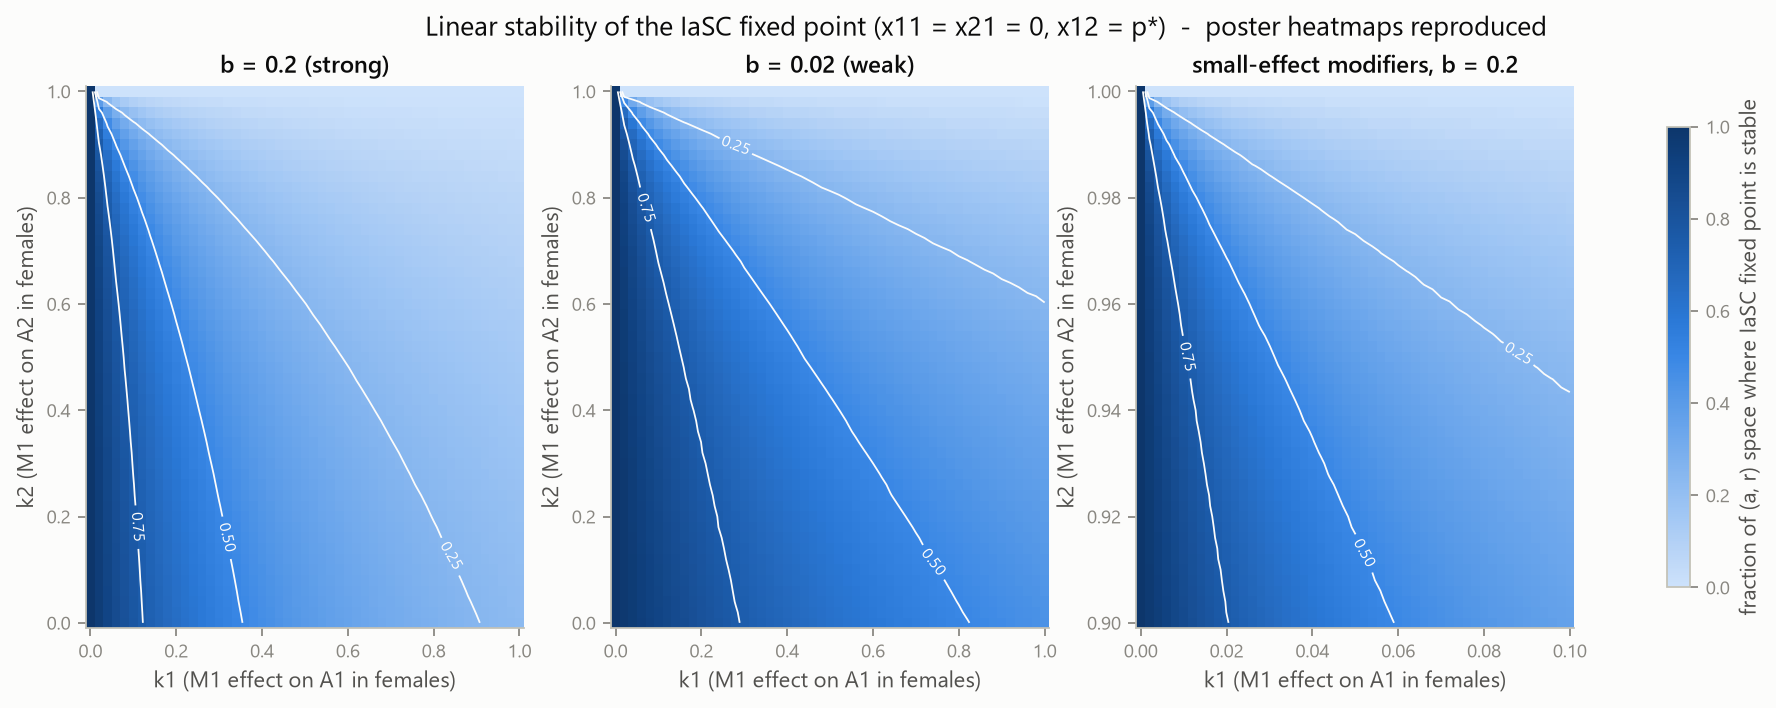
\includegraphics[width=0.85\textwidth]{P1_stability_heatmaps.png}
\caption{Poster reproduction: fraction of the $(a,r)$ rectangle in which IaSC is stable.}\end{figure}
\begin{figure}[H]\centering
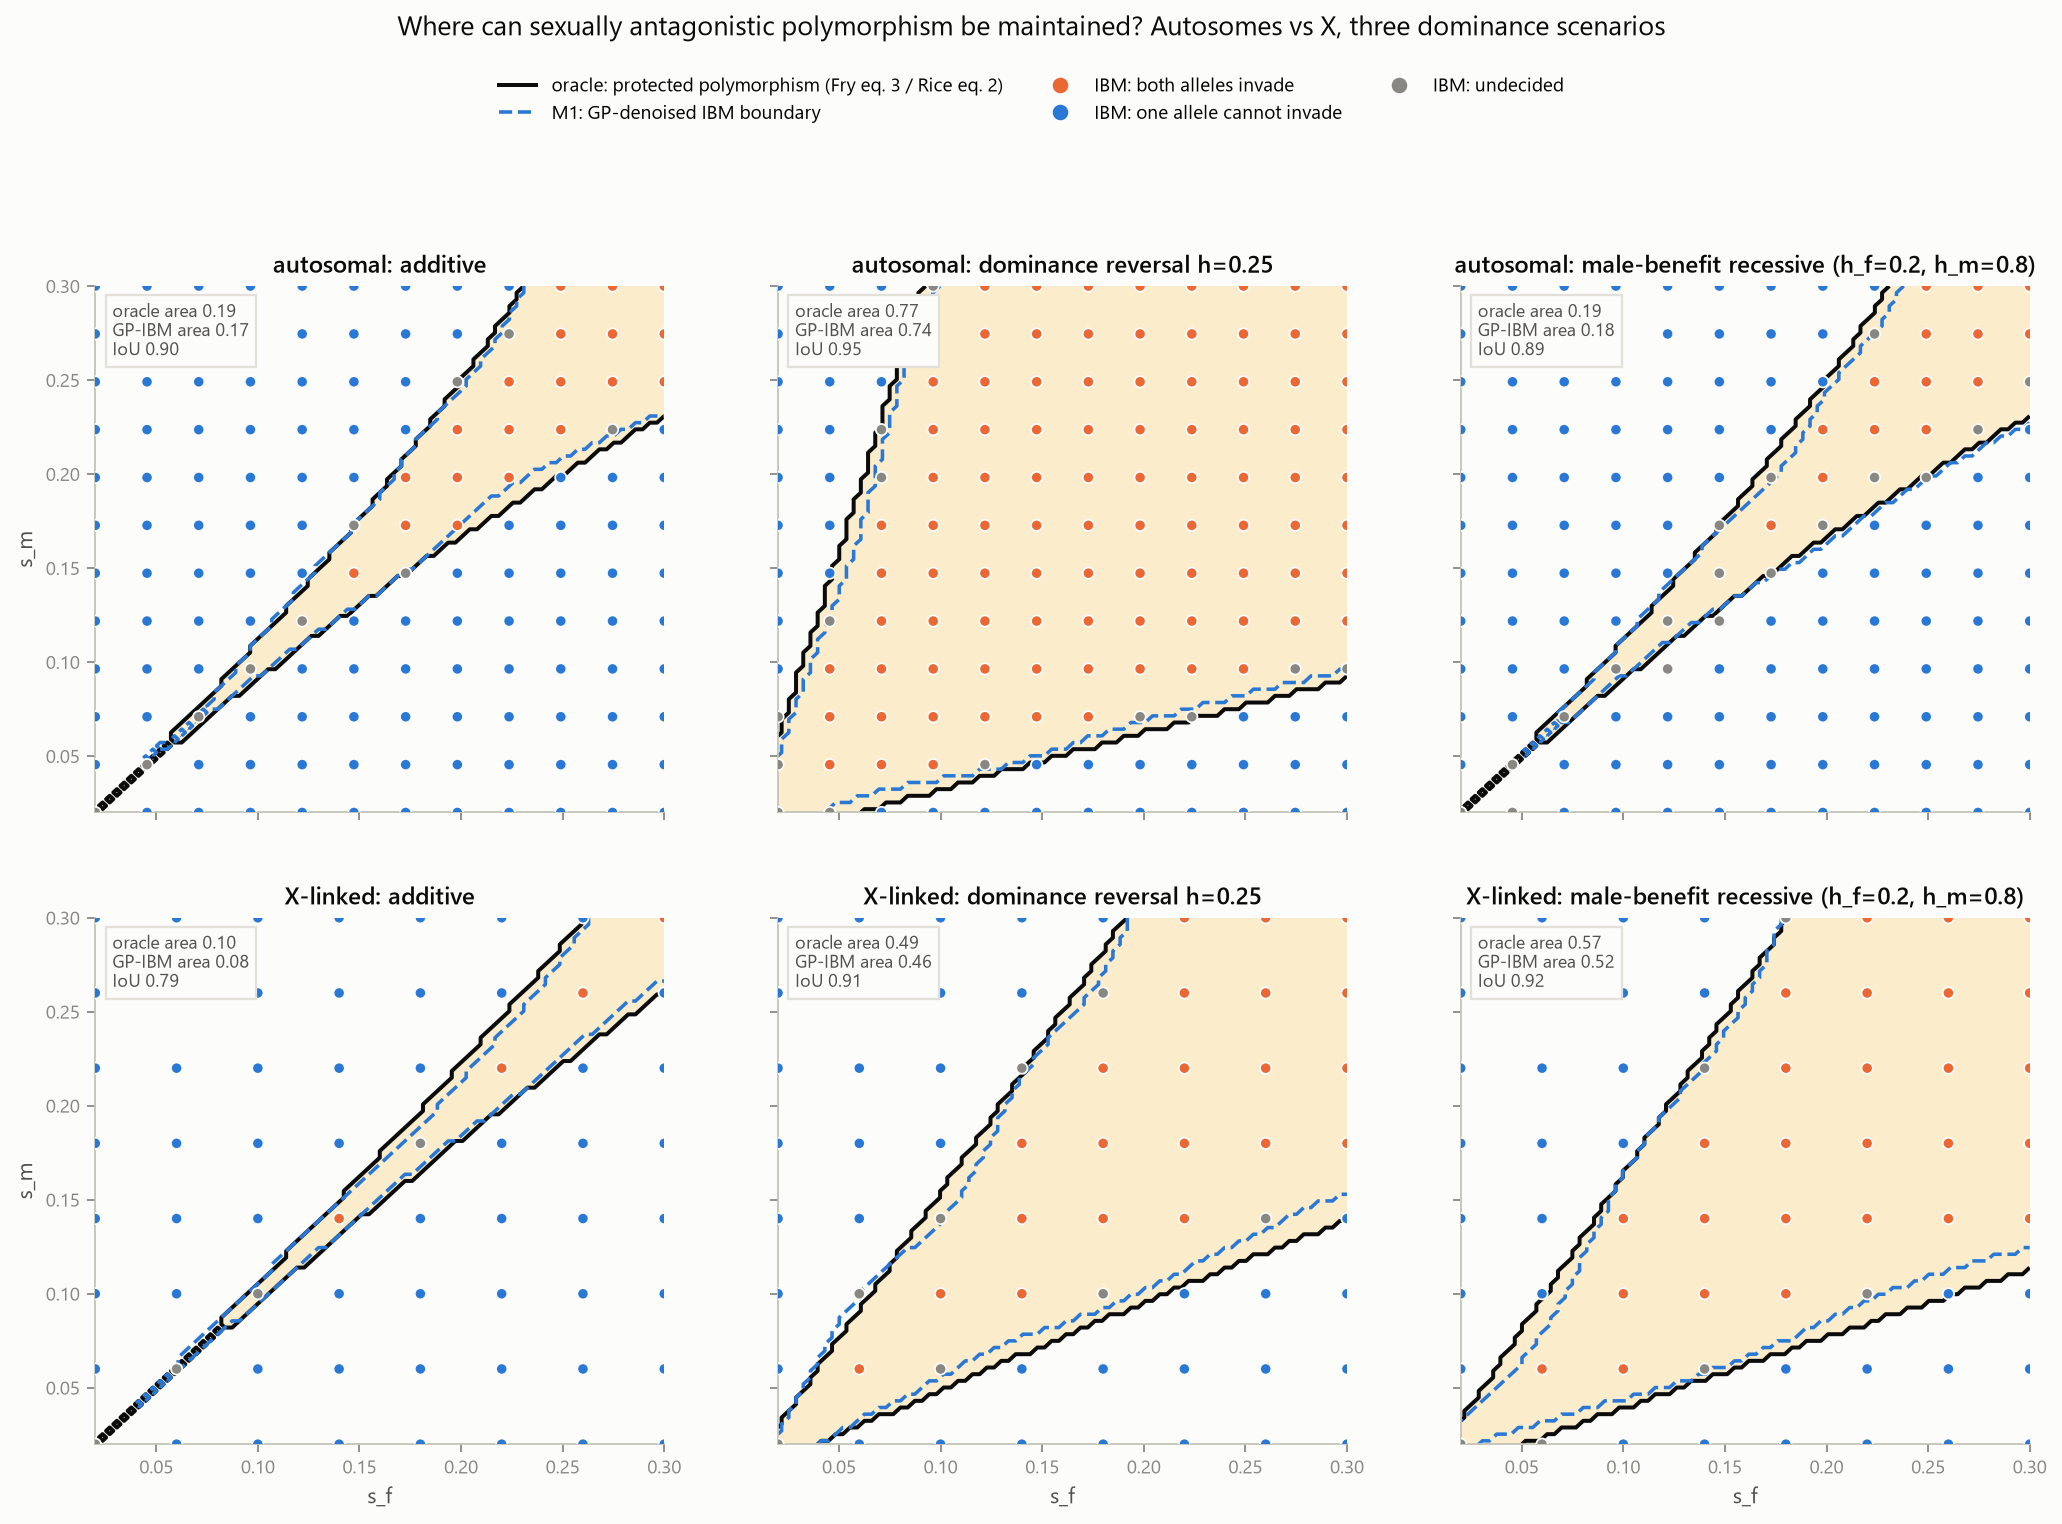
\includegraphics[width=\textwidth]{E1_E2_polymorphism_maps.png}
\caption{Protected polymorphism: oracle region (shaded), GP-denoised \IBM\ boundary (dashed), \IBM\ cell verdicts.}\end{figure}

\section{Project 2: target 1 recomputed from raw data}
\begin{tabularx}{\textwidth}{lXX}\toprule
Statistic (MB / E / FB) & Paper \claimA & Recomputed \claimB\\\midrule
$\rwg$ & 0.3805 / 0.4027 / 0.2515 & identical\\
SA proportion & 0.3097 / 0.2986 / 0.3742 & identical\\
Across-SR $r$, males & 0.5567 / 0.6995 / 0.5415 & identical\\
$r$(MB)$-r$(FB) & 0.129 [$-0.072$, 0.351] & 0.129 [$-0.090$, 0.330]\\\bottomrule
\end{tabularx}

\section{Project 2: LH-like populations and the emulated assay}
\begin{tabularx}{\textwidth}{p{3.1cm}XlX}\toprule
Regime & Assay $\rwg$ (MB/E/FB) & True hemigenome $r$ & Verdict\\\midrule
shared (10\% SA) & +0.093 / +0.095 / +0.076 & +0.15 & matches sign, matches ordering, misses magnitude\\
sex-limited null & $-0.049$ / $-0.058$ / $-0.046$ & $-0.05$ & null holds\\
true SA (80\%) & $-0.79$ / $-0.75$ / $-0.58$ & $-1.00$ & null holds (collapsed)\\
LH-like ($f_\mathrm{SA}$ 0.06, SC 0.93) & $\approx+0.45$ (E) & +0.47 \ldots\ +0.73 & matches sign and magnitude\\\bottomrule
\end{tabularx}

\begin{itemize}
\item \textbf{Out-of-sample checks} (shared regime):
  \begin{itemize}
  \item male across-SR correlations: 0.51 / 0.68 / 0.49 against 0.557 / 0.700 / 0.542 (match);
  \item female across-SR correlations: 0.87--0.89 against 0.75--0.84 (too high). There is no G$\times$SR in the model, which suggests real G$\times$SR in female fitness.
  \end{itemize}
\item \textbf{Power} (LH-like architecture). Attenuation alone predicts an MB$-$FB gap of $+0.09$ against the observed $+0.129$. It is significant with 39 lines in only 15\% of studies; 320 lines give 45\%; FB lowest in 57\% $\to$ 95\%.
\end{itemize}

\begin{figure}[H]\centering
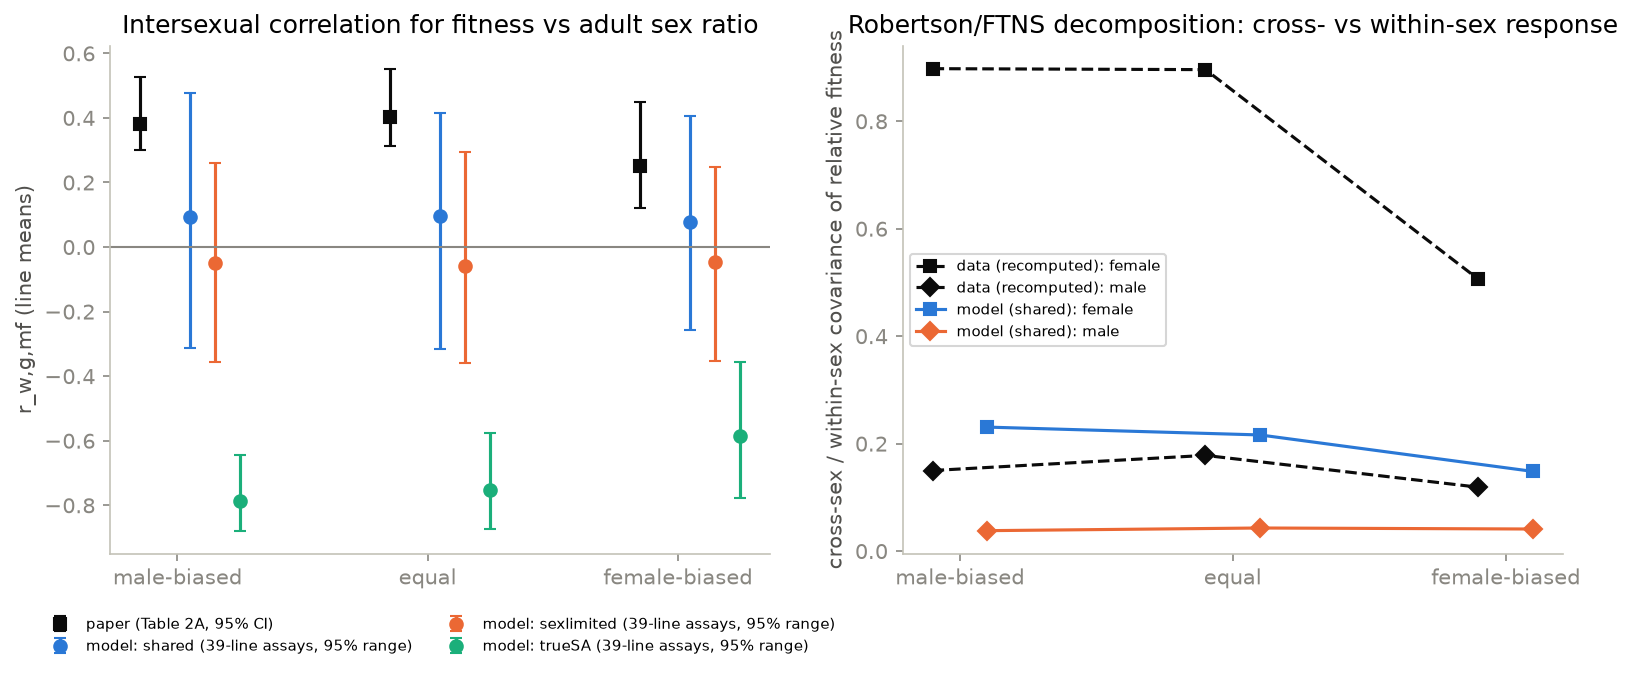
\includegraphics[width=\textwidth]{fig_r_vs_sexratio_and_robertson.png}
\caption{Left: $\rwg$ vs sex ratio, paper and model regimes. Right: Robertson/FTNS ratio of cross- to within-sex covariance of relative fitness, data vs model.}\end{figure}

\section{Project 2: Robertson layer}\label{sec:res-robertson}
The ratio of cross- to within-sex covariance of relative fitness, the cross-sex share of each sex's predicted response (sex-specific FTNS), is shown in the right panel above.
\begin{itemize}
\item \textbf{Data} \claimB: females 0.90 / 0.90 / 0.51 (MB / E / FB); males 0.15 / 0.18 / 0.12.
\item \textbf{Model} (shared regime): females 0.23 / 0.22 / 0.15; males 0.04 / 0.04 / 0.04.
\item \textbf{Verdict:} matches sign; matches ordering for females (FB lowest); misses magnitude, which scales with $r$.
\item Trait-level covariances (Am Nat 2025) are \emph{not identified}.
\end{itemize}

\section{Project 2: contrast reconciliation \claimC}
\begin{tabularx}{\textwidth}{XlX}\toprule
Architecture & 39-line assay $r$ & Comparable published value\\\midrule
$f_\mathrm{SA}$ 0.06, SC 0.93 & +0.45 & LH +0.40\\
$f_\mathrm{SA}$ 0.02--0.08, SC 0.24--0.55 & +0.10 to +0.14 & Ruzicka +0.15; Collet UCL +0.21\\
$f_\mathrm{SA}$ 0.10--0.14, SC 0.12--0.39 & $-0.24$ to $-0.27$ & Chippindale $-0.30$\\
$f_\mathrm{SA}$ 0.19, SC 0.85 & $-0.35$ (populations $-0.79$, +0.09) & Innocenti \& Morrow $-0.52$; Collet UU $-0.41$\\
$f_\mathrm{SA}\ge0.22$ & collapse, $r\to-1$ & --\\\bottomrule
\end{tabularx}

\noindent Which assumption moves the sign:
\begin{enumerate}
\item the SA share of mutational input, conditional on the concordant share;
\item replicate history near the collapse boundary;
\item \emph{not} sampling: the SD of $\hat r$ is 0.14 at 40 lines and 0.05 at 223;
\item \emph{not} HRI alone, which gives only negative $r$ with population means $\le0.15$ in magnitude at 0.1--1\,M.
\end{enumerate}

\section{Project 2: HRI (target 4)}
\begin{tabularx}{\textwidth}{l>{\raggedright\arraybackslash}X>{\raggedright\arraybackslash}X>{\raggedright\arraybackslash}X>{\raggedright\arraybackslash}X}\toprule
Map length & Paper median & Model, $\lambda=1$, all 6 (no filter) & Model, $\lambda=2$, non-collapsed & Drosophila setting \claimC\\\midrule
0.001\,M & $-0.115$ & $-0.184\pm0.052$ & $-0.26$ (2/6 left) & $-0.28$ (3/6)\\
0.01\,M & $-0.125$ & $-0.071\pm0.061$ & $-0.15$ & $-0.01$ (4/6, unreliable)\\
0.1\,M & $-0.07$ (mean $-0.078$) & $-0.042\pm0.041$ & $-0.086$ & $-0.133$\\
1\,M & $-0.02$ & -- & $-0.038$ & $-0.049$\\
10\,M & 0 & -- & +0.003 & +0.017\\\bottomrule
\end{tabularx}
\begin{itemize}
\item \textbf{$\lambda=1$ (the paper's own scale).} None of the 18 replicates collapses ($V_f$ 0.014--0.037). The means agree with the paper's medians within sampling error (Welch $p=0.25$, 0.42, 0.44 at 0.001, 0.01, 0.1\,M), and keep its ordering. These are the headline values; the $\lambda=2$ column gives upper bounds.
\item \textbf{Trend.} Spearman(log map, $r$) = +1. \emph{Matches ordering.}
\item \textbf{$\mu$ sweep.} $r=-0.054$, $-0.086$, $-0.149$, $-0.183$ for $\mu=5,7,9,13\times10^{-7}$. \emph{Matches ordering.}
\item \textbf{Variance.} $V_f$ rescaled back to $\lambda=1$ is 0.022 (paper about 0.02).
\end{itemize}
\begin{figure}[H]\centering
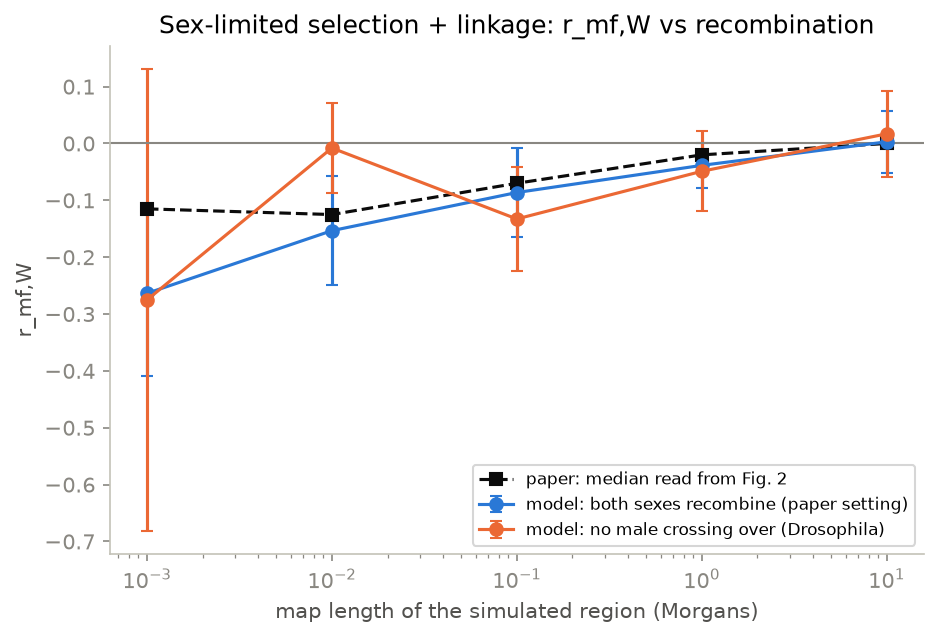
\includegraphics[width=0.75\textwidth]{fig_r_vs_recombination.png}
\caption{$\rmf$ vs map length: paper medians, model with both sexes recombining, model without male recombination.}\end{figure}
\begin{figure}[H]\centering
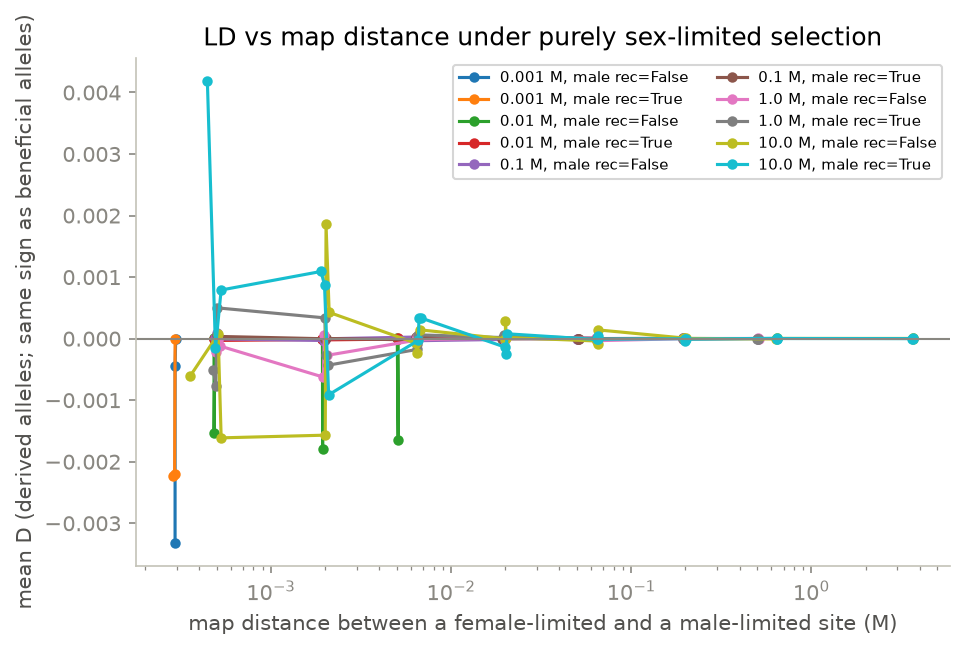
\includegraphics[width=0.75\textwidth]{fig_ld_vs_distance.png}
\caption{Signed LD between female-limited and male-limited derived alleles vs map distance.}\end{figure}

\section{Project 2: modifiers (target 5)}
The authors' code was re-executed on its exact grid \claimB.

\noindent\begin{tabularx}{\textwidth}{XXl}\toprule
Claim & Model & Verdict\\\midrule
perfect modifier 95.7\% & 97.2\% & misses magnitude (+0.015)\\
$k_2=1$: $>85\%$ & min 91.6\% & matches\\
monotone in $k_2$ & 100\% of rows & matches ordering\\
non-monotone in $k_1$ & minimum at $k_1=0.2$ & matches ordering\\
X $>$ A overall & 0.492 vs 0.222 & matches ordering\\
X resolves imperfect modifiers & $k_2$ 0.3--0.6: A 0.018, X 0.415 & matches ordering\\
A $>$ X at very high $k_2$ & A$-$X $=-0.016$ & does not match\\\bottomrule
\end{tabularx}
\begin{figure}[H]\centering
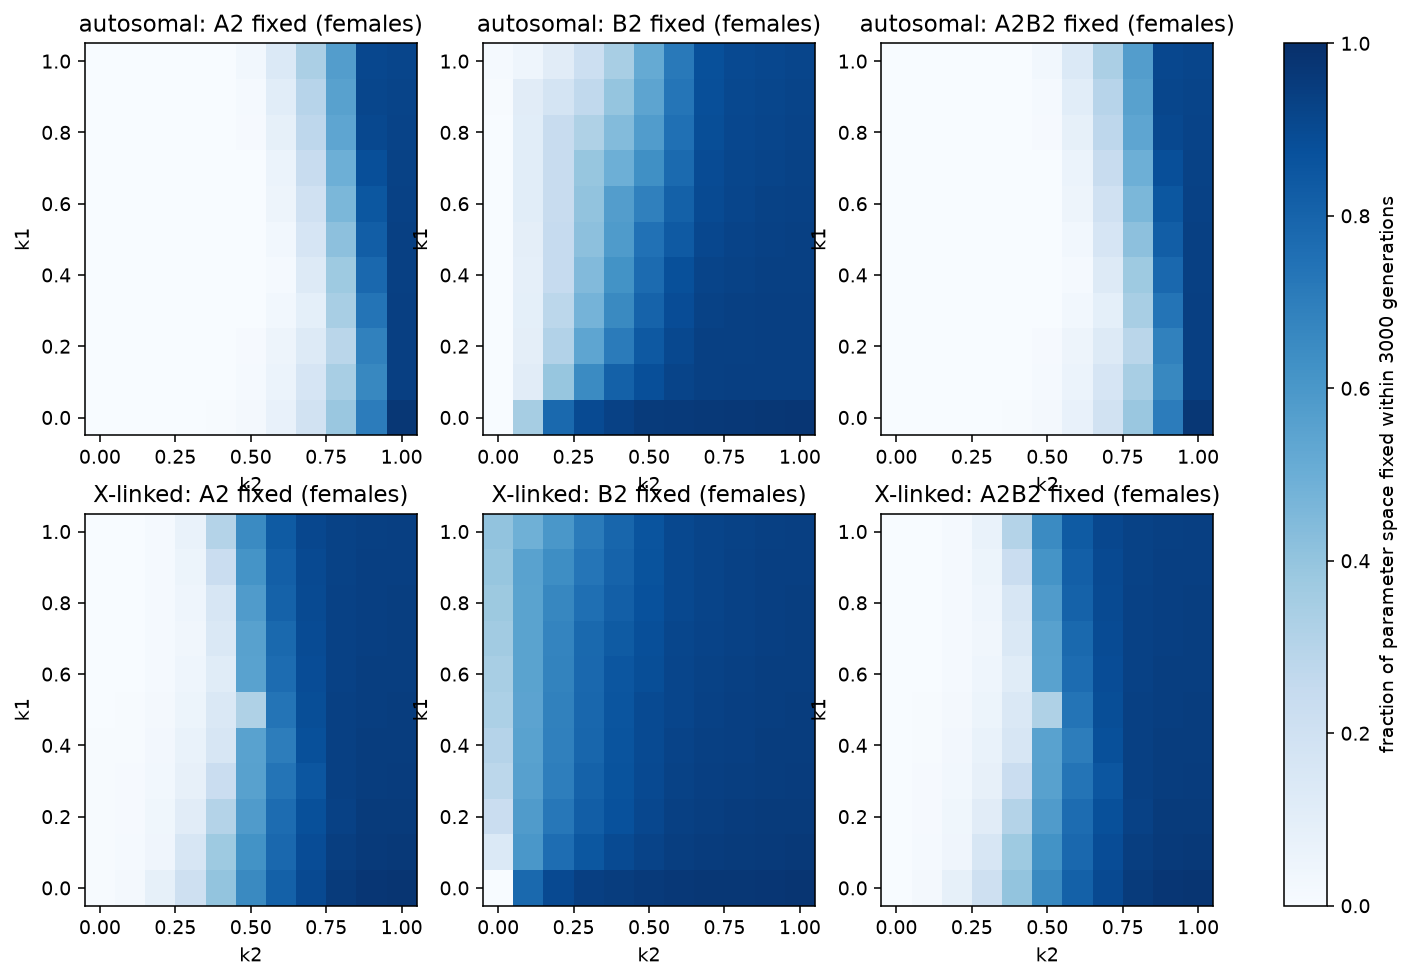
\includegraphics[width=0.85\textwidth]{fig_modifier_fraction.png}
\caption{Fraction of parameter space resolved, autosome vs X.}\end{figure}

\section{Project 2: the distinguishing experiments \claimC}
\begin{tabularx}{\textwidth}{Xcccc}\toprule
Population & $r(k{=}0)$ & $r(k{=}16)$ & $r_\mathrm{LE}$ & Power (200+200 lines)\\\midrule
HRI 0.01\,M & $-0.20$ & $-0.16$ & $\approx0$ & 0.08\\
HRI 0.1\,M & $-0.13$ & $-0.08$ & $\approx0$ & 0.08\\
LH sex-limited & $-0.08$ & $-0.08$ & +0.01 & 0.10\\
LH shared & +0.15 & +0.25 & +0.24 & 0.22\\
LH true SA & $-1.00$ & $-1.00$ & $-0.75$ & 0.97\\\bottomrule
\end{tabularx}
\begin{itemize}
\item \textbf{Recombination test.} All of the HRI-type $r$ is LD, yet feasible numbers of meioses do not break it.
\item \textbf{N-dependence} (0.1\,M, $\lambda=1$ parameters). $r=-0.128/-0.144/-0.042$ at $N=625/1250/2500$. The direction is as HRI predicts but the trend is not monotone, and about 31 populations per $N$ would be needed for 80\% power.
\end{itemize}
\begin{figure}[H]\centering
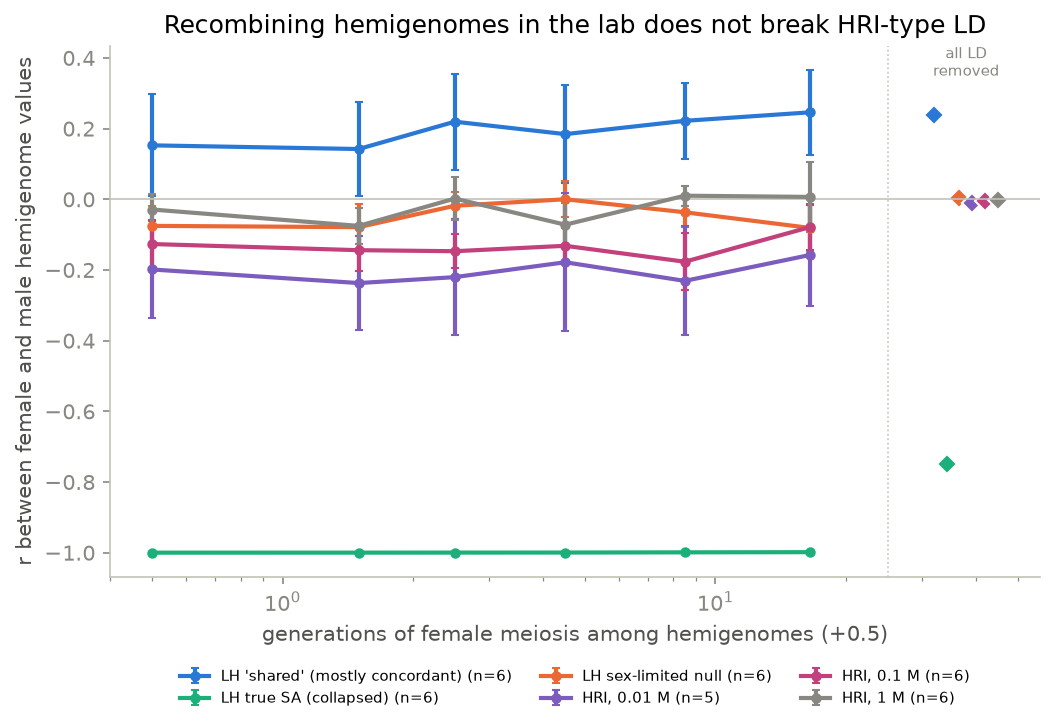
\includegraphics[width=0.8\textwidth]{fig_distinguish_default.png}
\caption{$r$ after $k$ generations of female meiosis among hemigenomes; diamonds: all LD removed.}\end{figure}

\chapter{Extension: male mate choice and telegony (Chinmay 2019)}\label{ch:chinmay}

\section{Problem}
Temura Chinmay Krishna Yadav's BS--MS thesis (IISER Mohali, April 2019, supervisor N.\,G.\ Prasad) used the IUS experimental-evolution populations to ask two questions:
\begin{enumerate}
\item Do sperm-depleted males prefer sham-infected over \emph{P.\ entomophila}-infected (decapitated) females? Measured as courts first (CF), courtship latency (CL) and courts most (CM).
\item Does a female's first mate (the stepfather) change the infection survival of offspring sired by her second mate (telegony)?
\end{enumerate}
Both answers were null. This is \emph{not} a sexually-antagonistic-allele study. The genetic core of Chapter~\ref{ch:build2} cannot emit any of these statistics, and a test (A5) fails if it ever does.

\textbf{Contrast papers}
\begin{itemize}
\item Khan \& Prasad 2013 (\emph{Serratia}, intact females): a positive control.
\item Wittman \& Fedorka 2015 (decapitated females): choice survives decapitation.
\item Morrow \emph{et al.}\ 2003: a constraint on mate harm.
\item Crean \emph{et al.}\ 2014: the \emph{Telostylinus} telegony template.
\item Byrne \& Rice 2006: independent calibration of male choosiness.
\item Gupta's 2016 PhD thesis: the fecundity and clearance data Chinmay cites.
\end{itemize}

\section{Three optional modules (all off by default)}
\begin{description}
\item[A: quality + choice] (\code{extensions/quality.py}, \code{choice.py})
  \begin{itemize}
  \item A female has infection $I$, a genotype-specific clearance and fecundity $F=F_0(1-\kappa I)$. Perceived quality is $q=F/F_0$, or 1 if the cue is off.
  \item Courtship follows the softmax kernel $P(\text{court }1)=e^{\beta q_1}/(e^{\beta q_1}+e^{\beta q_2})$, with $\beta=\beta_0\times$depletion.
  \item A minute-by-minute two-choice vial gives CF, CL and CM. A group mating vial reproduces the Khan and Byrne \& Rice assays.
  \end{itemize}
\item[B: harm] (\code{harm.py}) Female response to harm $\eta$: remating hazard $\times(1+\rho\eta)$ and egg-laying rate $\times(1-\lambda\eta)$, with $\rho,\lambda\ge0$ (Morrow's signs). A closed-form invasion analysis gives the boundary $m^*(\eta)$ of competitive mating success needed for a harmful mutant to spread.
\item[C: telegony] (\code{telegony.py})
  \begin{itemize}
  \item A compartmentalisation flag decides whether a first-male semen state can reach the ova. It is on for \emph{Drosophila} (author hypothesis); off gives the \emph{Telostylinus} template.
  \item The non-genetic state exists only when the module is on.
  \item Mother's curse is never used as a stand-in for telegony.
  \end{itemize}
\end{description}

\textbf{Configuration.} Parameters live in \code{config/ius.yaml} and \code{khan.yaml}, each with a provenance and grade. The repository has no pyyaml, so a small YAML-subset loader was written. The statistics (factorial ANOVA, log-rank, Cox Wald) are hand-written and checked against scipy.

\section{Source facts the build depends on}
\begin{itemize}
\item \textbf{Thesis Table 3.2.} The p-values are the \emph{smaller one-sided} binomial tail, verified on all 16 rows. Two-sided they are all $\ge0.11$.
\item \textbf{Gupta 2016 Table 8.1(e).} No infection effect on fecundity ($p=0.27$), but measured at 96\,h on survivors. Chinmay tested choice at 12--14\,h, so $\kappa=0$ is a switch, not a measurement.
\item \textbf{Khan Table 5.} Bias scores 0.447--0.478; fecundity about 40\% lower in infected females (gives $\kappa_\text{Khan}=0.4$).
\item \textbf{Byrne \& Rice 2006.} Fecundity 69.30 vs 25.06 ($\Delta q=0.638$). Vials with more large females mated: 22/32 for non-depleted males, 57/72 for depleted males.
\end{itemize}

\section{Calibration: why the independent route matters}
The spec froze $\beta_0$ by its A2 threshold (sham courted first in more than 60\%), which gave $\beta_0=2.5$. The audit (Chapter~\ref{ch:audit}) classed this as fitted. Calibrating on Byrne \& Rice alone gives:
\begin{itemize}
\item $\beta_\text{depleted}=0.59$ (95\% range 0.30--0.88) and $\beta_\text{non-depleted}=0.32$;
\item a blind Khan prediction of 0.480 (range 0.449--0.502) against the observed 0.463.
\end{itemize}
On the raw scale the error is $+3.7\%$. The no-choice baseline 0.500 is also within 10\%, however, so the informative metric is the effect against 0.5: predicted 0.020, observed 0.037. The calibrated model implies $P(\text{sham first})=0.53$ for Khan, so the spec's A2 threshold is inconsistent with independent data. It is met only by the labelled override \code{config/spec_a2.yaml}.

\section{Results (calibrated defaults)}
\begin{tabularx}{\textwidth}{>{\raggedright\arraybackslash}p{4.2cm}>{\raggedright\arraybackslash}X>{\raggedright\arraybackslash}p{3.8cm}}\toprule
Result & Model & Evidence type\\\midrule
Courts-first null & share 0.50; all 4 blocks n.s.\ in 85\% of studies & by construction ($\kappa=0$)\\
Latency, courts-most nulls & consistent & by construction\\
Courts-most SD, held-out blocks & 0.405 vs 0.423 ($-4\%$) & out-of-sample (within study)\\
Khan bias & 0.475; effect about 2/3 of observed & out-of-sample\\
A3: Chinmay design with a 40\% cost & detected in 73\% of studies (pooled test) & prediction\\
Fecundity cost excluded by Chinmay's null & $\kappa\le0.44$ (0.30--0.86) & calibrated\\
Wittman \& Fedorka CM 0.64 & unreachable (maximum 0.575 at $\kappa=1$) & out-of-sample: misses\\
Harm-only mutant & lost ($s=-0.17$) & by construction (Morrow's signs)\\
Harm + mating success & spreads above $m^*(0.5)=0.20$ & boundary result\\
Stepfather effect & none ($p$ uniform) & by construction\\
Telegony sex effect & not reproducible from independent data & rejected (H10)\\\bottomrule
\end{tabularx}

\section{Smallest missing assays}
\begin{enumerate}
\item \textbf{Fecundity of the exact choice-vial females}, measured from 12--14\,h after infection.
  \begin{itemize}
  \item A cost near 0 supports ``no fecundity difference''.
  \item A cost of 40\% or more means males are not perceiving it, or are less sensitive than Byrne \& Rice imply.
  \end{itemize}
\item \textbf{A replicated telegony block.}
  \begin{itemize}
  \item One block detects a stepfather log-hazard shift of $\pm0.2$ with 74\% power.
  \item Four blocks detect $\pm0.1$ with 80\% power.
  \item Both figures use a baseline mortality set by us.
  \end{itemize}
\end{enumerate}

\section{Building it}
\begin{lstlisting}[style=sh]
python scripts/calibrate_byrne_rice.py        # independent beta calibration (Byrne & Rice only)
python scripts/run_chinmay_calibrated.py      # A3, kappa bound, W&F under calibrated beta
python scripts/run_chinmay.py                 # outputs/chinmay_comparison.csv (+ evidence_type column)
python scripts/run_chinmay_power.py           # telegony power, choice bound
python analysis/hypothesis_tests.py           # outputs/hypothesis_tests.csv
NUMBA_NUM_THREADS=2 python -m pytest -q tests/   # 29 tests
\end{lstlisting}

\chapter{Audit: leakage, circularity, triviality, and hypothesis tests}\label{ch:audit}
A match between model and paper means little if the model was given the answer. This chapter classifies every comparison by how its result was obtained, records the fixes made, and applies formal tests of whether the model predicts or explains each result.

\section{Evidence types}
\begin{description}
\item[By construction:] the assumptions guarantee the result. Example: $\kappa=0$ makes courtship choice exactly 50/50.
\item[Input echo:] a value is taken from the target and compared with itself. Example: the sign of the telegony sex effect.
\item[Fitted:] tuned to the target, or to a threshold derived from it. Example: the spec $\beta_0$.
\item[Calibrated:] partly uses the scored data. Example: the variance calibration of the hemiclone assay.
\item[Existential:] true for chosen parameter values. Example: a harm-plus-competitiveness mutant spreading.
\item[Out-of-sample:] no target information is used. Example: Khan's bias predicted from Byrne \& Rice.
\end{description}

\section{Main findings and fixes}
\begin{longtable}{p{4.6cm}p{5.2cm}p{5.4cm}}\toprule
Finding & Diagnosis & Fix / status\\\midrule\endhead
Courtship and telegony nulls & by construction ($\kappa=0$; stepfather effect $=0$) & labelled ``consistent, not evidence''\\
$\beta_0$ chosen to pass A2, then moved after seeing Khan & fitted; data peeking & calibrated on Byrne \& Rice only; spec value moved to a compliance override\\
Courts-most spread calibrated on the scored table & calibration leakage & calibrate on blocks 1--2, test on 3--4 ($-4\%$)\\
``Fecundity cost $<10\%$'' bound & circular (used the spec $\beta$) & withdrawn; calibrated bound $\kappa\le0.44$\\
Telegony sex effect & sign taken from the target & not scored; the independent test rejects it\\
Sex-ratio ordering (Manas) & echo: data-only attenuation gives E $>$ M $>$ F & labelled; test H13 added\\
SA proportion & identity $(1-r)/2$ & labelled\\
LH $+0.45$ & selected from 12 design points & labelled fitted; prior-predictive test H15\\
HRI collapse filter & defined post hoc & validated: 0/12 collapse at $\lambda=1$ at 0.001 and 0.01\,M (H18); $\lambda=1$ values now headline\\
Raw-scale ``within 10\%'' & the no-effect baseline also passes & effect sizes reported against the baseline\\\bottomrule
\end{longtable}

\section{Can magnitudes be brought within 10\%?}
Only one sign-matched quantity has a legitimate route: Khan's bias, through independent calibration. It is within 4\% on the raw scale, but that criterion is uninformative near 0.5. On the effect scale the prediction is about half to two-thirds of the observed effect, with the observation inside the predictive interval.
\begin{itemize}
\item Wittman \& Fedorka: no fecundity cost reaches CM 0.64.
\item Telegony sex effect: cannot be predicted without fitting to the target.
\item Latency genotype effects: not identified.
\end{itemize}
Forcing any of these within 10\% would mean fitting the scored data.

\section{Hypothesis tests}
\begin{itemize}
\item \textbf{Methods.} Predictive p-values from 300 replicate simulations, using the analytic F and $\chi^2$ tails where the null is exact. Likelihood ratios between competing hypotheses. Benjamini--Hochberg FDR over the substantive tests only. An informativeness column for each test.
\item \textbf{Files.} Results are in \code{outputs/hypothesis_tests.csv}; the narrative is in \code{docs/08_hypothesis_tests.md}.
\end{itemize}

\begin{tabularx}{\textwidth}{>{\raggedright\arraybackslash}p{4.6cm}>{\raggedright\arraybackslash}X>{\raggedright\arraybackslash}p{3.6cm}}\toprule
Test & Result & Verdict\\\midrule
Chinmay courts-first: $\kappa=0$ vs $\kappa=0.4$ & LR $=3.4$ & no cost favoured, moderately\\
Khan: calibrated vs no-choice vs spec $\beta$ & LR 2.8 and 6.8 & weak evidence for the calibrated model\\
Khan between-vial SD implied by its CIs & 0.029 vs model 0.111 ($q=0.045$) & \textbf{rejected}: assay mechanics\\
Telegony sex $\chi^2=108$ with independent HR $=1$ & $p=2.5\times10^{-25}$ & \textbf{rejected}\\
Latency genotype effects & $p=0.009$, 0.011 ($q=0.07$) & tension (no mechanism)\\
Female across-SR correlations (Manas) & $p=0.017$ ($q=0.09$) & tension (no G$\times$SR)\\
Attenuation-only sex-ratio pattern (Manas) & disattenuated $r$ 0.47 / 0.48 / 0.35, $p\approx0.3$ & not rejected; low power\\
Manas $r_{w,g,mf}$ under the shared regime & $p$ 0.08--0.34 & consistent but uninformative\\
HRI mean at 0.1\,M ($\lambda=1$) & $p=0.44$ & consistent; underpowered ($n=6$)\\
HRI at 0.001 / 0.01\,M ($\lambda=1$, no filter) & $-0.184$ / $-0.071$ vs $-0.115$ / $-0.125$; $p=0.25$ / 0.42 & consistent; collapse filter justified\\
Khan under the spec-frozen $\beta$ & 0.413 vs 0.463, $p=0.028$ ($q=0.13$) & tension: spec $\beta$ too strong\\
Courts-most held-out SD & $p=0.08$ & consistent\\\bottomrule
\end{tabularx}

\textbf{Bottom line.}
\begin{itemize}
\item Where the model makes genuine out-of-sample predictions, the data agree in direction, with weak to moderate evidence.
\item Where the data contain structure the model lacks, it is rejected or in tension: assay dispersion, the sex effect on survival, genotype effects, and female genotype $\times$ sex-ratio interaction.
\item Many ``matches'' carry no information, because they are guaranteed by construction or because the model's predictive interval is very wide.
\end{itemize}

\chapter{Troubleshooting protocols}\label{ch:trouble}

\section{General protocol}
\begin{enumerate}
\item \textbf{Reproduce at the smallest scale.} Use the quick profile, one replicate, one thread (\code{NUMBA_NUM_THREADS=1}). Numba errors are clearer if you temporarily run the Python function un-jitted (\code{func.py_func(...)}).
\item \textbf{Check invariants before results.}
  \begin{itemize}
  \item allele frequencies within $[0,1]$;
  \item $V_f$ close to $\lambda^2\times0.02$;
  \item the number of segregating sites well below the site capacity;
  \item no NaN in calibrations.
  \end{itemize}
\item \textbf{Compare against a known answer:}
  \begin{itemize}
  \item a test in \code{tests/};
  \item the analytic layer;
  \item the published raw-data recomputation.
  \end{itemize}
\item \textbf{When a result looks too good or too bad} ($r=-1.000$ exactly; $V$ in the thousands; a perfect match), suspect a degenerate state or a bug before believing it.
\item \textbf{Change one thing at a time} and keep the failed output under a new name (e.g.\ \code{hri_runs_lambda4_partial.csv}). Failures are diagnostics.
\end{enumerate}

\section{Catalogue of problems we met}
\begin{longtable}{p{3.6cm}p{5.0cm}p{6.6cm}}
\toprule
\textbf{Symptom} & \textbf{Cause} & \textbf{Fix}\\\midrule\endhead
\label{tr:lambda}$\rmf\approx-1$ in most replicates; $V_f$ in the thousands; about 15,000 segregating sites & Rescaling artefact at $\lambda=4$ (and some short-map replicates at $\lambda=2$). Haplotypes split into a female-lethal, male-favoured class carried only through sons (a neo-Y) and its complement. $N V_g$ and the ratchet speed are not rescaling-invariant & Diagnose: 2-means clustering of haplotype loads; between-class share 0.993. Lower $\lambda$; flag replicates with $V_f/\lambda^2>0.1$ as collapsed, report and exclude them; validate the headline at $\lambda=1$\\
Same collapse in LH regimes with many SA mutations & SA benefits accumulate on non-recombining male-transmitted autosomes; unbounded $\exp(BV)$ fitness & Use SA benefit ratio $b<1$; restrict $f_\mathrm{SA}\le0.2$; report the collapse as a finding\\
$V$ in the thousands even without linkage & $b=1$ makes additive SA alleles exactly neutral averaged over the sexes; they drift and accumulate & $b=0.5$ (\S5.6)\\
\label{tr:hemiY}True hemigenome $r=0.997$ (implausible) & Hemigenome sampling included Y slots (empty X) & Sample from males: X = maternal slot, autosome = a random one of two\\
Paternal autosomes never sampled & Autosome tied to the X slot & Draw the autosome slot independently (clone-generator protocol)\\
Calibration overflow; Poisson $\lambda$ too large & Unstandardised BVs with $\lambda$-inflated variance & Standardise BVs by competitor SD; bound $\beta\le5$; optimise on the log scale\\
Recomputed $r=0.382/0.419/0.236$, not 0.3805/0.4027/0.2515 & Arcsine transform applied as the Methods describe (F12) & Untransformed proportions reproduce all 12 values exactly; keep a flag \code{ARCSINE_MALES}\\
Bootstrap takes about 8\,h & Pandas loop of \code{concat}/\code{groupby} per resample & Vectorised \code{np.bincount} version (45\,s for 10k); verify with the identity resample\\
Percentile CIs sit below the estimate & Vial resampling attenuates correlations & Also report the basic interval; state that the published CI method is not identified\\
\label{tr:ne}Neutral $N_e$ test fails (+17\%) & Expectation $e^{-\sigma^2}$ is the large-$N$ limit; at $n=75$ parents per sex the exact value is 0.399, not 0.368 & Monte-Carlo the finite-$N$ expectation; 12 replicates; 3\,SE tolerance\\
\label{tr:gp}GP emulator ``consistent'' with everything; flat sensitivity & GP learned noise: CV RMSE 0.30 vs replicate SD 0.15; strong between-population variance & Gate the emulator on CV RMSE $<1.5\times$ replicate SD; otherwise report ``not identified'' and use the design table\\
GP boundary denoiser inflates regions (IoU 0.004) & Zero-variance cells collapse the length scale & Variance floor, length-scale lower bound = grid spacing, tanh response\\
Design sweep wastes runs & Most of $f_\mathrm{SA}\in[0,0.5]$ is collapsed & Pilot the range; restrict to the informative region\\
Recombination experiment shows no effect & HRI LD is between tightly linked loci, and $k$ meioses break it only if $kc\gtrsim1$ & Report as a negative result; use magnitude and sign plus $N$-dependence\\
\label{tr:slim}SLiM fails to build with MSVC & gnulib needs POSIX configure & Use MSYS2/WSL/conda on another machine; keep SLiM scripts; make the cross-check skip gracefully\\
\label{tr:errno22}\code{OSError: [Errno 22] Invalid argument} saving a PNG & Windows file lock (viewer, preview pane, antivirus) on the target file & Write to a temp file, then \code{os.replace}, retrying with back-off\\
Long job killed after 2\,h & Agent tool's background limit & Launch detached: \code{Start-Process -WindowStyle Hidden bash chain.sh}\\
Stopping jobs killed the controlling shell & Kill-by-command-line match also matched the shell running the kill command & Match on PIDs, or on patterns absent from your own command\\
Two Python processes per job & Windows venv \code{python.exe} is a launcher that spawns the real interpreter & Expected; check parent-child PIDs before assuming duplicates\\
Edited bash chain while it ran misbehaves & Bash reads scripts incrementally & Never edit a running script; write a new chain\\
\texttt{\textbackslash n} became literal newlines, or \texttt{\textbackslash b} became a backspace (LaTeX: ``Unicode character U+0008'') in generated files & The shell layer collapsed \texttt{\textbackslash\textbackslash} to \texttt{\textbackslash} inside inline scripts (PowerShell/heredoc escaping) & Write patch scripts to files with an editor tool and run them; scan outputs for control characters\\
TOML mixture keys are strings & TOML keys are always strings & Convert digit keys to \code{int} on load\\
\code{NUMBA_NUM_THREADS} ignored & Set after numba was imported & Set the env var in the config module imported first\\
Figure legend hides data; 13 cycled colours & Too many series; default colour cycle & At most 6 series in fixed colours; legend below the axes; jitter coincident markers\\
``No state allocated'' test fails although the attribute was deleted & A dataclass field with a default lives on the class, so \code{del obj.attr} leaves it visible & Do not declare optional state as a field; attach it only when the module is on\\
Predictive p-values never below 0.016 & Monte Carlo floor $1/(R+1)$ & Use the analytic F or $\chi^2$ tail when the null is exact; increase $R$\\
FDR hides real rejections & Rows that cannot fail (by construction, echoes) dilute the family & Restrict the FDR family to substantive tests\\
A fitted parameter looks like a prediction & Tuned to a threshold or after viewing the target & Calibrate on an independent study; test that fitting code never reads the target\\
Trait standing SD 0.03--0.09, not the intended 0.15 & Infinite-sites formula $V=4NU\sigma^2$ ignores finite-sites saturation (one-way mutation; mean derived frequency $\approx0.2$) & Neutral burn-in: rescale the effects to the target SD in the ancestor; keep the raw run as a sensitivity case\\
Faster-clearing genotypes had a higher early cost & Cost anchored at 96\,h and extrapolated backwards with $e^{c(96-t)}$ & Model load decaying from infection, $e^{-ct}$; normalise the ancestor at 96\,h; test monotonicity\\
Male-expressed trait mean drifts to 1.15 & Reference mean taken over both sexes; the X counts once in males & Normalise each trait in the sex that expresses it\\
Model predicting a large F passes as ``consistent'' & One-sided upper-tail predictive p & Use two-sided tails when the model can miss in either direction\\
X-linked invasion condition off by 2 & Scan of Parsons' ``note added in proof'' & Derive it yourself; trust internal consistency over the scan\\\bottomrule
\end{longtable}

\section{Resource incidents: a checklist before every heavy launch}
\begin{enumerate}
\item List Python processes and their parents; identify your own.
\item Check free RAM. A $\lambda=4$ population set peaked at 4\,GB; $\lambda=2$ LH runs at about 0.3\,GB per process.
\item Confirm that no other heavy job of yours is running (one at a time).
\item Launch at below-normal priority with \code{cpu-2} threads.
\item Set a monitor on the stage log that greps for progress \emph{and} failure signatures (\code{Traceback|Error|exit}).
\end{enumerate}

\chapter{Heuristics, nuances, caveats and limits}\label{ch:heur}

\section{Heuristics that worked}
\begin{enumerate}
\item \textbf{Reproduce the raw data first.} The arcsine finding (F12) only surfaced because we insisted on 4-decimal agreement. Agreement to 2 decimals hides pipeline differences.
\item \textbf{Reconstruct under-specified models by elimination.} Enumerate the plausible life cycles and keep the one whose closed form matches the published formula.
\item \textbf{Re-run authors' code rather than re-derive their figures.} For the modifier paper, an exact compiled re-implementation of their supplement (with quirks) scores their claims; a ``cleaned'' version would not.
\item \textbf{Calibrate to variances, predict correlations.} This turns the hemiclone emulator into a genuine test: the male across-sex-ratio correlations and the MB$-$FB gap were predicted, not fitted.
\item \textbf{Run the nulls.} The sex-limited null exposed the deterministic sex-differential LD term ($r\approx-0.05$ even without HRI).
\item \textbf{Scale to the diffusion variable.} The $Ns$ input made the neural emulator extrapolate; generic inputs did not.
\item \textbf{Measure $N_e$ from the simulator itself} before using diffusion theory: $N_e/N\approx0.9$ under random survival.
\item \textbf{Pilot before sweeping.} A 2-point pilot of a design range saves hours, for example by revealing collapse above $f_\mathrm{SA}\approx0.2$.
\item \textbf{Keep failed runs.} The $\lambda=4$ partial results became the rescaling diagnostic.
\end{enumerate}

\section{Nuances that change conclusions}
\begin{itemize}
\item \textbf{Two different ``$r_\mathrm{mf}$''s.}
  \begin{itemize}
  \item The HRI preprint's $\rmf$ correlates breeding values over \emph{pooled female and male genotypes}.
  \item Hemiclonal $\rwg$ correlates female and male values of the \emph{same haploid genome}.
  \end{itemize}
  When males do not recombine, the sexes can differ genetically. Then the pooled estimator reads intersexual differentiation as negative covariance: $-0.94$ vs a hemigenome $r$ of $-0.06$ in collapsed populations. Even in stable LH-like populations, the pooled $r$ was $-0.41\ldots0$ against a hemigenome $r$ of $+0.47\ldots+0.73$.
\item \textbf{Male recombination matters.}
  \begin{itemize}
  \item SLiM's default lets both sexes recombine.
  \item With $r_m=0$, sex-limited selection creates negative LD along entire chromosomes deterministically, and HRI bias is 1.3--1.5$\times$ stronger at 0.1--1\,M.
  \end{itemize}
\item \textbf{Attenuation is enough to make $r$ depend on sex ratio.} Lower genetic signal-to-noise at FB (smaller calibrated $\beta$) lowers $\hat r$ without any change in genetic architecture. The published ordering is consistent with attenuation alone and with a real G$\times$SR; 39 lines cannot tell them apart.
\item \textbf{The SA proportion is not extra evidence.} For scaled and centred line means, the 45\textdegree\ rotation gives $\mathrm{Var}(w_a)/(\mathrm{Var}(w_a)+\mathrm{Var}(w_c))=(1-r)/2$ exactly. The published SA proportions equal $(1-\rwg)/2$ to 4 decimals. Treat ``higher SA proportion at FB'' as the same observation as ``lower $r$ at FB'', not as independent support (\S\ref{ex:rot}).
\item \textbf{LD can mask concordance.} In LH-like regimes the indirect term was \emph{negative}: removing LD raised $r$ from $+0.15$ to $+0.24$.
\item \textbf{Between-population variance dominates.} Replicate populations of one architecture differed by up to 0.9 in $r$ near the collapse boundary. A single population's $r$, which is all any real study measures, is a weak guide to its architecture.
\item \textbf{The SA benefit ratio is not innocuous.} Additive SA with benefit = cost is neutral on average over the sexes, which is a knife-edge. Results for ``true SA'' regimes depend on $b$ and on the unbounded $\exp(BV)$ fitness.
\end{itemize}

\section{Audit rules (learned the hard way)}
\begin{enumerate}
\item Report effect sizes against a null baseline. ``Within 10\%'' on proportions near 0.5 is passed by the no-effect model.
\item Tag every comparison with its evidence type: by construction, input echo, fitted, calibrated, existential, or out-of-sample.
\item Calibrate free sensitivities on independent studies with measured inputs (here Byrne \& Rice 2006), never on the scored target or on thresholds derived from it.
\item Hold out part of the data whenever you must calibrate on the target study.
\item Freeze exclusion rules before looking, or report filtered and unfiltered summaries side by side.
\item Ask of every ``consistent'' verdict how wide the predictive interval was; a wide interval makes the verdict uninformative.
\end{enumerate}

\section{Caveats}
\begin{warnbox}[Read before citing any number from this work]
\begin{itemize}
\item \textbf{Rescaling.} HRI magnitudes at $\lambda=2$ are about 2$\times$ too strong. Only the $\lambda=1$ runs (0.001, 0.01 and 0.1\,M; 6 replicates each, SE about 0.05) are trusted for magnitude; elsewhere trust sign and ordering only.
\item \textbf{Architecture is an input, not an estimate.} No paper reports the mutation-class mixture of LH or LH$_\mathrm{M}$. The design table shows which mixtures \emph{could} produce each published $r$, not which one did.
\item \textbf{Phenomenological sex ratio.} IeSC is represented only as a selection-intensity multiplier. There are no harm, persistence or resistance traits, so trait-level questions (thesis Ch.\ 4, Am Nat 2025) are not identified.
\item \textbf{No dominance reversal or balancing selection in the \IBM.} SA polymorphism there is maintained only by mutation--selection--drift; balancing selection lives only in the analytic modifier layer.
\item \textbf{Single autosome + X.} Real hemigenomes span 2 large autosomes plus the X; whole-genome $r$ averages over chromosomes.
\item \textbf{Emulator.} The GP failed validation, so no inference rests on it.
\item \textbf{Modifier heatmaps.} The cell values are unpublished; only the quoted percentages and orderings were scored.
\end{itemize}
\end{warnbox}

\section{What the models cannot predict}
\begin{enumerate}
\item The absolute LH value of $\rwg$, which needs the unknown mixture (L1).
\item Whether the sex-ratio effect is attenuation or a real G$\times$SR change (L2).
\item The Am Nat 2025 Robertson covariances (L3; the paper is inaccessible and the trait data are not deposited).
\item Why the LH and LH$_\mathrm{M}$ estimates differ (L4). The model shows what \emph{could} differ: SA share and history; not sampling, not HRI alone.
\item Exact HRI magnitudes at map lengths without $\lambda=1$ runs (1 and 10\,M), and anything finer than about $\pm0.1$ anywhere (L5).
\end{enumerate}

\section{Distinguishing SA from HRI: the final position \claimC}
\begin{itemize}
\item \textbf{Recombining hemigenomes in the lab} has no power: HRI LD is between tightly linked loci.
\item \textbf{Varying $N$} works in direction but needs about 31 replicate populations per $N$ for $|r|\approx0.1$.
\item \textbf{Practical criterion: magnitude and sign.}
  \begin{itemize}
  \item HRI and sex-limited LD give only negative $r$. Population means are $|r|\lesssim0.15$ at 0.1--1\,M, and single populations reach $-0.26$.
  \item A positive $r$ (LH) cannot be HRI-driven.
  \item $-0.41$ and $-0.52$ exceed realistic-map HRI.
  \item Chippindale's $-0.30$, and anything in $[-0.3,0]$, is not identified.
  \end{itemize}
\item \textbf{Genomic $r_\mathrm{LE}$} (direct term only, from per-locus effect estimates) separates the regimes perfectly in silico, but needs hundreds of densely genotyped lines.
\end{itemize}

\section{Open questions for the authors}
\begin{itemize}
\item \textbf{Poster:} the intended life cycle; the domain of ``fraction of parameter space''; the initial condition of the ``away from fixed point'' panel; the $r$ used in the perturbation panel.
\item \textbf{BMC 2022:} the bootstrap CI method, and whether the line-mean statistics used untransformed male proportions (F12).
\item \textbf{HRI preprint:} the replicate-level values behind Fig.\ 2, and whether the pooled-sex estimator was checked for intersexual differentiation.
\end{itemize}

\appendix
\chapter{Environment and pinned versions}\label{app:env}
\begin{tabularx}{\textwidth}{lX}\toprule
Python & 3.14.6\\
numpy / numba / scipy & 2.5.3 / 0.68.0 / 1.18.1\\
scikit-learn / pandas / matplotlib & 1.9.1 / 3.0.6 / 3.11.2\\
openpyxl / psutil / pytest & 3.1.5 / 7.2.2 / 9.1.1\\
project 1 extras & sympy 1.14, pyarrow, pyopencl 2026.1.4 (GPU, optional)\\
SLiM (scripts only) & 5.2\\
OS / hardware & Windows 10, Ryzen 5 2500U (4C/8T), 32\,GB RAM, Radeon RX 560X 4\,GB\\\bottomrule
\end{tabularx}

\chapter{Parameter table (project 2)}
\begin{longtable}{p{4.6cm}p{7.2cm}p{3.4cm}}\toprule
Parameter & Value & Provenance\\\midrule\endhead
HRI: $N$, generations & 2,500; 25,000 & [paper]\\
HRI: region, $\mu$ & 1\,Mb; $7\times10^{-7}$ (sweep 5--13$\times10^{-7}$) & [paper]\\
HRI: map lengths & 0.001--10\,M & [paper]\\
DFE & reflected $\Gamma$(0.3, 0.05), $h=0.5$ & [paper]\\
Fitness & $\exp(BV+N(0,1))$ & [paper]\\
Sample & 250\,F + 250\,M & [paper]\\
Male crossing over & none (Drosophila setting) / both sexes (paper setting) & [bio] / [paper]\\
LH census & 960\,F + 960\,M & [paper] BMC 2022\\
LH autosome map, X map & 1.0\,M, 0.66\,M (female) & [ours] / [bio]\\
LH mutation mixtures & shared, sex-limited, true SA; design $f_\mathrm{SA}\in[0,0.2]$ & [ours]\\
SA benefit/cost $b$ & 0.5 & [ours]\\
Sites & 32,768 autosomal + 8,192 X & [ours]\\
$\lambda$ & quick 10, default 2, full 1 & [ours], measured\\
Assay lines, sex ratios & 39; 24:8, 16:16, 8:24 & [paper]\\
Female assay & 2 focal, 7 vials $\times$ 2 days & [paper]\\
Male assay & 5 vials $\times$ 7 scored females $\times$ 2 days; 1:3 & [paper]\\
Eggs per female, offspring per scored female & 25, 20 & [ours]\\
$\beta_s(SR)$, noise & calibrated to line variance + within-cell CV$^2$ & [data]\\\bottomrule
\end{longtable}

\chapter{Command reference}
\begin{lstlisting}[style=sh]
# project 2 (run inside manas_sa/)
python analysis/recompute_bmc2022.py 10000           # target 1 from raw data + bootstrap
python scripts/run_modifier.py                       # target 5, authors' grid
python scripts/run_lh.py --profile default           # LH regimes + assays (saves pops/*.npz)
python scripts/run_design.py --profile default --points 12 --reps 2
python scripts/run_emulator.py --profile default
python scripts/run_hri.py --profile default          # target 4 grid (saves pops)
python scripts/run_lambda_check.py --maps 0.1 --lams 1 --reps 6
python scripts/run_power_lhlike.py --profile default
python scripts/run_distinguish.py --profile default
python scripts/run_ne_check.py --Ns 625,1250 --reps 6
python scripts/make_comparison.py                    # table, coverage, figures
python scripts/calibrate_byrne_rice.py               # independent choice calibration
python scripts/run_chinmay_calibrated.py             # Chinmay consequences of the calibration
python scripts/run_chinmay.py                        # Chinmay comparison (+ evidence types)
python scripts/run_chinmay_power.py                  # telegony power, choice bound
python analysis/hypothesis_tests.py                  # formal tests, outputs/hypothesis_tests.csv
python scripts/run_all.py --profile default [--only lh,design] [--force]
NUMBA_NUM_THREADS=1 python -m pytest -q tests/test_core.py
\end{lstlisting}

\chapter{Rebuild checklist}
\begin{enumerate}
\item[$\square$] Environment pinned; \code{NUMBA_NUM_THREADS} set before import; below-normal priority.
\item[$\square$] Source map written: access status, extracted tables, flags.
\item[$\square$] Raw-data recomputation matches the paper to 4 decimals (F12 resolved).
\item[$\square$] Analytic layer: one-step LD halving; the sex-limited $D$ sign test; modifier claims reproduced.
\item[$\square$] Engine tests: Haldane, neutral $\pi$ (exact finite-$N$ target), zero leakage.
\item[$\square$] $\lambda$-sensitivity measured; collapse diagnostic in place.
\item[$\square$] Hemigenomes sampled from males (X maternal, random autosome).
\item[$\square$] Calibration on variances only; instrument frozen.
\item[$\square$] Nulls run (sex-limited, true SA) and reported.
\item[$\square$] Design pilot run before the full sweep; emulator gated on CV.
\item[$\square$] Power computed at an architecture matching the published $r$.
\item[$\square$] Comparison table uses the fixed verdict words; coverage table written.
\item[$\square$] Figures checked by eye; at most 6 series per plot.
\end{enumerate}

\chapter{Glossary}
\begin{description}[style=nextline]
\item[Hemigenome] A haploid genome (X + major autosomes) propagated intact via clone-generator crosses.
\item[IaSC / IeSC] Intra- / interlocus sexual conflict.
\item[HRI] Hill--Robertson interference: selection at linked loci in a finite population reduces the efficacy of selection and builds repulsion LD.
\item[Direct / indirect term] The pleiotropic and LD parts of $\mathrm{COV}(BV_f,BV_m)$.
\item[$r_\mathrm{LE}$] $r$ after removing all LD (site-wise permutation); the direct-term-only correlation.
\item[$\lambda$] The rescaling factor ($N/\lambda$; $U,R,s\times\lambda$).
\item[Collapse] A degenerate state with female-lethal haplotype classes transmitted through sons; $V_f/\lambda^2>0.1$, $r\to-1$.
\item[Instrument] The frozen calibrated assay parameters $(\beta_s(SR),\sigma)$.
\item[Oracle] The deterministic implementation of a paper's equations.
\item[Zero leakage] The rule that the \IBM\ never uses the oracle's mathematics.
\end{description}

\chapter*{References}
\addcontentsline{toc}{chapter}{References}
\small
\begin{itemize}[leftmargin=*,label={}]
\item Abbott JK, Morrow EH (2011) Obtaining snapshots of genetic variation using hemiclonal analysis. \emph{Trends Ecol Evol} 26:359--368.
\item Chippindale AK, Gibson JR, Rice WR (2001) Negative genetic correlation for adult fitness between sexes reveals ontogenetic conflict in \emph{Drosophila}. \emph{PNAS} 98:1671--1675.
\item Collet JM \emph{et al.}\ (2016) \emph{Evolution} (PMC5069644); values from the primary text.
\item Comeron JM, Ratnappan R, Bailin S (2012) The many landscapes of recombination in \emph{Drosophila melanogaster}. \emph{PLoS Genet} 8:e1002905.
\item Connallon T, Clark AG (2010) Sex linkage, sex-specific selection, and the role of recombination in the evolution of sexually dimorphic gene expression. \emph{Evolution} 64:3417--3442.
\item Fry JD (2010) The genomic location of sexually antagonistic variation: some cautionary comments. \emph{Evolution} 64:1510--1516.
\item Geeta Arun M, Chechi TS, Meena R, Bhosle SD, Srishti, Prasad NG (2022) Investigating the interaction between interlocus and intralocus sexual conflict using hemiclonal analysis in \emph{Drosophila melanogaster}. \emph{BMC Ecol Evol} 22:38. doi:10.1186/s12862-022-01992-0.
\item Geeta Arun M (2025) Tie that binds -- Hill-Robertson interference can produce signals of sexual antagonism even in the absence of sexually antagonistic selection. \emph{bioRxiv} doi:10.1101/2025.01.08.632022.
\item Geeta Arun M \emph{et al.}\ (2025) \emph{Am Nat} 206(6):552--568. Not accessible to us; title and content not quoted.
\item Havird JC \emph{et al.}\ (2019) Selfish mitonuclear conflict. \emph{Curr Biol} 29:R496--R511.
\item Innocenti P, Morrow EH (2010) The sexually antagonistic genes of \emph{Drosophila melanogaster}. \emph{PLoS Biol} 8:e1000335.
\item Kidwell JF \emph{et al.}\ (1977) Regions of stable equilibria for models of differential selection in the two sexes under random mating. \emph{Genetics} 85:171--183.
\item Kimura M (1962) On the probability of fixation of mutant genes in a population. \emph{Genetics} 47:713--719.
\item Morrow EH, Arnqvist G, Pitnick S (2003) Adaptation versus pleiotropy: why do males harm their mates? \emph{Behav Ecol} 14:802--806.
\item Owen ARG (1953) A genetical system admitting of two distinct stable equilibria under natural selection. \emph{Heredity} 7:97--102.
\item Parsons PA (1961) The initial progress of new genes with viability differences between sexes and with sex linkage. \emph{Heredity} 16:103--107.
\item Rice WR (1984) Sex chromosomes and the evolution of sexual dimorphism. \emph{Evolution} 38:735--742.
\item Rice WR (1987) The accumulation of sexually antagonistic genes as a selective agent promoting the evolution of reduced recombination between primitive sex chromosomes. \emph{Evolution} 41:911--914.
\item Ruzicka F \emph{et al.}\ (2019) bioRxiv preprint 117176; values from the primary text.
\item Samant MA (2022) ``The ties that bind'': investigating the interaction between interlocus and intralocus sexual conflict using \emph{Drosophila melanogaster}. PhD thesis, IISER Mohali.
\item Samant M, Moitra P, Sinha S, Prasad NG. A two-locus haploid model for the resolution of intra-locus sexual conflict (poster, IISER Mohali).
\item Singh, Jain, Geeta Arun \& Prasad (2023) Nature and location of modifier alleles determine the resolution of intralocus sexual conflict. \emph{bioRxiv} doi:10.1101/2023.10.25.564090.
\end{itemize}

\end{document}
